\documentclass[usenames,dvipsnames]{beamer}

%& PACKAGES
\usepackage{graphicx}
\usepackage{amsmath,amsfonts,amssymb,amsthm}
\usepackage{mathtools}
\usepackage[noend]{algorithmic}
\usepackage{algorithm}
\usepackage{environ}
\usepackage{xcolor}
\usepackage{caption}
\usepackage{multicol}
\usepackage{array}
\usepackage[algo2e,vlined,ruled]{algorithm2e}
\usepackage{hyperref}
\usepackage{tcolorbox}
\usepackage{wasysym}
\usepackage{transparent}
\usepackage{relsize}
\usepackage{appendixnumberbeamer}
\usepackage[export]{adjustbox}
\usepackage{wrapfig}
\usepackage[absolute,overlay]{textpos}
\usepackage[utf8]{inputenc}
%\usepackage[texcoord, grid, gridcolor=red!10, subgridcolor=green!10, gridunit=cm]{eso-pic}
\usepackage{tikzit}
\usepackage{adjustbox}
\usepackage{pgfgantt}
\usepackage{tikz}
\usepackage{pgfplots}
\usetikzlibrary{shapes,fit,arrows,backgrounds,positioning,fadings,shadows,intersections, pgfplots.fillbetween,shapes.misc,automata,patterns}

\tikzset{
	cross/.style={
		cross out,
		draw=black,
		minimum size=2*(#1-\pgflinewidth),
		inner sep=0mm,
		outer sep=0mm
	},
	cross/.default={1mm} % default radius
}

\hypersetup{
	colorlinks=false,
	urlcolor=cyan,
	citecolor=black
}

%& BEAMER SETTINGS
\usetheme{default}
% \usecolortheme{seagull}

\setbeamertemplate{blocks}[rounded]% Rounded blocks

\useoutertheme[subsection=false]{miniframes}

\makeatletter
\let\beamer@writeslidentry@miniframeson=\beamer@writeslidentry
\def\beamer@writeslidentry@miniframesoff{%
  \expandafter\beamer@ifempty\expandafter{\beamer@framestartpage}{}% does not happen normally
  {%else
    % removed \addtocontents commands
    \clearpage\beamer@notesactions%
  }
}
\newcommand*{\miniframeson}{\let\beamer@writeslidentry=\beamer@writeslidentry@miniframeson}
\newcommand*{\miniframesoff}{\let\beamer@writeslidentry=\beamer@writeslidentry@miniframesoff}
\makeatother

\setbeamerfont{footnote}{size=\tiny}
\setbeamerfont{frametitle}{size=\large}

%& BEAMER

\beamertemplatenavigationsymbolsempty
\setbeamertemplate{footline}[frame number]

\newcommand{\sectiontitle}{}
%\newcommand{\sectionnumber}{}
\newcommand{\newsection}[1]{\section{#1}\renewcommand{\sectiontitle}{#1}}

\newcommand{\mdpgray}{black!10}

\newcommand{\citesize}{\tiny} % \scriptsize

\newcommand{\ftitleintro}[1]{%
	\frametitle{#1}%
}%
\newcommand{\ftitlei}[1]{%
	\frametitle{\makebox[1.13\textwidth]{#1\hfill\includegraphics[height=5mm, trim={0mm 2mm 0mm 0mm}]{images/numbers/i}}}%
}%
\newcommand{\ftitleii}[1]{%
	\frametitle{\makebox[1.13\textwidth]{#1\hfill\includegraphics[height=5mm, trim={0mm 2mm 0mm 0mm}]{images/numbers/ii}}}%
}%
\newcommand{\ftitleiii}[1]{%
	\frametitle{\makebox[1.13\textwidth]{#1\hfill\includegraphics[height=5mm, trim={0mm 2mm 0mm 0mm}]{images/numbers/iii}}}%
}%

% Contributions drawing
\newcommand{\cla}{red}
\newcommand{\clb}{cyan}
\newcommand{\clc}{orange}
\newcommand{\arrowcolor}{orange!30}
\newcommand{\thk}{thick}
\newcommand{\cone}[3]{
	\draw [draw=none, fill=#3, opacity=0.25] plot [] coordinates {(#1, #2) (#1 + 9mm, #2 + 8mm) (#1 + 9mm, #2 - 8mm)};
	
%	\draw[dashed] (#1, #2) -- (#1 + 9mm, #2 + 8mm);
%	\draw[dashed] (#1, #2) -- (#1 + 9mm, #2 - 8mm);
	
	\draw (#1, #2) node [oltadot, color=\clb, fill=white] {};
}
\newcommand{\finalcone}[3]{
	\draw [draw=none, fill=#3, opacity=0.25] plot [] coordinates {(#1, #2) (#1 + 9mm, #2 + 8mm) (#1 + 9mm, #2 - 8mm)};
	
	\draw (#1, #2) node [oltadot, color=\clb, fill=white] {};
}
\newcommand{\lipub}[4]{ % color thickness x y
	\draw [#1, #2] (#3, #4) -- (#3-1, #4+2.8);
	\draw [#1, #2] (#3, #4) -- (#3+1, #4+2.8);
}
\newcommand{\lipcone}[4]{ % color thickness x y fillcolor
	\def\ratio{0.35}
	\draw [#1, #2, dashed, name path = A] (#3-\ratio*1, #4-\ratio*2.8) -- (#3+\ratio*1, #4+\ratio*2.8);
	\draw [#1, #2, dashed, name path = B] (#3+\ratio*1, #4-\ratio*2.8) -- (#3-\ratio*1, #4+\ratio*2.8);
	\tikzfillbetween[of = A and B]{#1, opacity=0.2};
}


%\begin{tcolorbox}[title=Planification]
%	TODO
%\end{tcolorbox}

\newtcolorbox{mdpbox}[1][]{
	notitle,
	height=1.3cm,
	colframe=green!60!black,
	colback=green!20!white,
	boxrule=-0.1mm,
	valign=center,
	valign lower=center,
	halign=center,
	#1
}

%\newcommand{\sectiontitle}{#1}
%\newcommand{\setsectiontitle}[1]{\renewcommand{sectiontitle}{#1}}

%& TEXTS
\newcommand{\ie}{\emph{i.e.}}
\newcommand{\eg}{\emph{e.g.}}
\newcommand{\vs}{\emph{vs.}}
\newcommand{\etc}{\emph{etc.}}
\newcommand{\wrt}{with respect to}
\newcommand{\st}{s.t.}
\newcommand{\ub}{upper bound}
\newcommand{\Ub}{Upper bound}
\newcommand{\cf}{closed-form}
\newcommand{\fp}{fixed-point}

\newcommand{\Qfun}{Q-function}
\newcommand{\Qval}{Q-value}

\newcommand{\ts}{tree search}
\newcommand{\Ts}{Tree search}
\newcommand{\TS}{Tree Search}
\newcommand{\ol}{open-loop}
\newcommand{\Ol}{Open-loop}
\newcommand{\cl}{closed-loop}
\newcommand{\Cl}{Closed-loop}

\newcommand{\wc}{worst case}
\newcommand{\Wc}{Worst case}
\newcommand{\ra}{risk averse}
\newcommand{\Ra}{Risk averse}

\newcommand{\ns}{non-stationary}
\newcommand{\Ns}{Non-stationary}
\newcommand{\NS}{Non-Stationary}
\newcommand{\nsty}{non-stationarity}
\newcommand{\nsties}{non-stationarities}
\newcommand{\Nsty}{Non-stationarity}
\renewcommand{\ne}{non-episodic}

\renewcommand{\l}{lifelong}
\renewcommand{\ll}{\l{} learning}
\newcommand{\lml}{\l{} {ML}}
\newcommand{\lrl}{\l{} {RL}}
\newcommand{\Lrl}{Lifelong {RL}}

\newcommand{\perspectiveintrosentence}{The content of this chapter suggests a few perspectives.}

\newcommand{\proofsentence}[2]{The proof of #1 is reported in the Appendix, Chapter~\ref{chap:app:proofs}, Section~\ref{#2}.}

\newcommand{\proofsentenceplural}[2]{The proofs of #1 are reported in the Appendix, Chapter~\ref{chap:app:proofs}, Section~\ref{#2}.}

%& Notations for larger symbols
\makeatletter
\newcommand{\vast}{\bBigg@{3}}
\newcommand{\Vast}{\bBigg@{5}}
\newcommand{\vastl}{\mathopen\vast}
\newcommand{\vastm}{\mathrel\vast}
\newcommand{\vastr}{\mathclose\vast}
\newcommand{\Vastl}{\mathopen\Vast}
\newcommand{\Vastm}{\mathrel\Vast}
\newcommand{\Vastr}{\mathclose\Vast}
\makeatother

%& MATHS
\newcommand*{\SET}[1]{\ensuremath{ \left\{ #1 \right\} }}
\newcommand*{\EXP}[1]{\ensuremath{ \mathbb{E} \left( #1 \right) }}
\newcommand*{\EXPLOW}[1]{\ensuremath{ \mathbb{E}_{#1} }}
\newcommand*{\EXPENS}[2]{\ensuremath{ \mathbb{E}_{#1} \left( #2 \right) }}
\newcommand{\argmax}{\operatornamewithlimits{argmax}}
\newcommand{\argmin}{\operatornamewithlimits{argmin}}
\newcommand{\MAX}[1]{\ensuremath{ \max \left\{ #1 \right\} }}
\newcommand{\MAXENS}[2]{\ensuremath{ \max_{#1} \left\{ #2 \right\} }}
\newcommand{\MIN}[1]{\ensuremath{ \min \left\{ #1 \right\} }}
\newcommand{\MINENS}[2]{\ensuremath{ \min_{#1} \left\{ #2 \right\} }}
\newcommand{\ARGMAX}[1]{\ensuremath{ \argmax \left\{ #1 \right\} }}
\newcommand{\ARGMAXENS}[2]{\ensuremath{ \argmax_{#1} \left\{ #2 \right\} }}
\newcommand{\ARGMIN}[1]{\ensuremath{ \argmin \left\{ #1 \right\} }}
\newcommand{\ARGMINENS}[2]{\ensuremath{ \argmin_{#1} \left\{ #2 \right\} }}
\DeclarePairedDelimiter{\ceil}{\lceil}{\rceil}
\newcommand{\bigo}{\ensuremath{\mathcal{O}}} % big O
\newcommand{\bigotilde}{\ensuremath{\tilde{\mathcal{O}}}}
\newcommand{\functionspace}[2]{\mathcal{F} \left( #1, #2 \right)}
\newcommand{\FUNCTION}[5]{
	\ensuremath{
		\begin{array}{llll}
			#1: & #2 & \rightarrow & #3 \\
			& #4 & \mapsto & #5
		\end{array}
	}
}

% Norms
\renewcommand{\L}{\ensuremath{\mathcal{L}}}
\newcommand{\absnorm}[1]{\ensuremath{ \left| #1 \right| }}
\newcommand{\nnorm}[2]{\ensuremath{ \left\lVert #1 \right\rVert_{#2} }}
\newcommand{\onenorm}[1]{\nnorm{#1}{1}}
\newcommand{\twonorm}[1]{\nnorm{#1}{2}}
\newcommand{\inftynorm}[1]{\nnorm{#1}{\infty}}

% Sets
\newcommand{\R}{\ensuremath{\mathbb{R}}}
\newcommand{\Z}{\ensuremath{\mathbb{Z}}}
\newcommand{\N}{\ensuremath{\mathbb{N}}}
\newcommand{\M}{\ensuremath{\mathcal{M}}}
\newcommand{\T}{\ensuremath{\mathcal{T}}}
\newcommand{\B}{\ensuremath{\mathcal{B}}}
\newcommand{\ball}[3]{\ensuremath{\B_{#1} \left( #2, #3 \right)}} % metric center radius
\newcommand{\intrange}[2]{\ensuremath{\left\{#1, \dots, #2\right\}}} % range of integers
\newcommand{\intrangeinfty}[2]{\ensuremath{\left\{#1, #2, \dots \right\}}} % infinite range of integers
\newcommand{\tuple}[2]{\ensuremath{\left( #1, #2 \right)}} % 2-uple
\newcommand{\threeuple}[3]{\ensuremath{\left( #1, #2, #3 \right)}} % 3-uple
\newcommand{\fouruple}[4]{\ensuremath{\left( #1, #2, #3, #4 \right)}} % 4-uple
\newcommand{\setcomplement}[1]{\ensuremath{{#1}^{c}}}

% Probabilities
\renewcommand{\Pr}{\ensuremath{\textbf{Pr}}}
\newcommand{\condPr}[2]{\ensuremath{\Pr \left( #1 \;\middle|\; #2 \right)}}
\renewcommand{\P}{\ensuremath{\mathcal{P}}} % set of probabilities

% Display
\newcommand{\mthspc}{\ensuremath{\,}}
\newcommand{\ms}{\ensuremath{\,}}
\newcommand{\eqspacing}{\ensuremath{\;}}
\newcommand{\rforall}{\ensuremath{\eqspacing\forall}}
\newcommand{\phleq}{\hphantom{\leq\text{ }}}
\newcommand{\phgeq}{\hphantom{\geq\text{ }}}
\newcommand{\pheq}{\hphantom{=\text{ }}}

%& MDP elements
\newcommand{\initstatedistrib}{\ensuremath{\P_0}}
\renewcommand{\S}{\ensuremath{\mathcal{S}}}
\newcommand{\A}{\ensuremath{\mathcal{A}}}
\newcommand{\cardinalactions}{\ensuremath{\SET{\text{Right, Up, Left, Down}}}}
\newcommand{\sa}{\ensuremath{\tuple{s}{a}}}
\newcommand{\SA}{\ensuremath{\S \times \A}}
\newcommand{\STA}{\ensuremath{\S \times \T \times \A}}
\newcommand{\nS}{\ensuremath{S}} % number of states
\newcommand{\nA}{\ensuremath{A}} % number of actions

\newcommand{\transition}{\ensuremath{T}}
\newcommand{\tra}[3]{\ensuremath{\transition{}_{#1 #3}^{#2}}} % s a s'
\newcommand{\trahat}[3]{\ensuremath{\hat{\transition{}}_{#1 #3}^{#2}}}
\newcommand{\trabar}[3]{\ensuremath{\bar{\transition{}}_{#1 #3}^{#2}}}
\newcommand{\trat}[4]{\ensuremath{\transition{}_{#2} \left( #4 \;\middle|\; #1, #3 \right)}} % s t a s'
\newcommand{\trahatt}[4]{\ensuremath{\hat{\transition{}}_{#2} \left( #4 \;\middle|\; #1, #3 \right)}}
\newcommand{\trabart}[4]{\ensuremath{\bar{\transition{}}_{#2} \left( #4 \;\middle|\; #1, #3 \right)}}
\newcommand{\tratildet}[4]{\ensuremath{\tilde{\transition{}}_{#2} \left( #4 \;\middle|\; #1, #3 \right)}}

\newcommand{\reward}{\ensuremath{r}}
\newcommand{\rew}[3]{\ensuremath{\reward{}_{#1 #3}^{#2}}} % s a s'
\newcommand{\rewhat}[3]{\ensuremath{\hat{\reward{}}_{#1 #3}^{#2}}}
\newcommand{\rewbar}[3]{\ensuremath{\bar{\reward{}}_{#1 #3}^{#2}}}
\newcommand{\rewhatbar}[3]{\ensuremath{\hat{\bar{\reward{}}}_{#1 #3}^{#2}}}
\newcommand{\rewt}[4]{\ensuremath{\reward{}_{#2} \left( #1, #3, #4 \right)}} % s t a s'
\newcommand{\rewhatt}[4]{\ensuremath{\hat{\reward{}}_{#2} \left( #1, #3, #4 \right)}}
\newcommand{\rewbart}[4]{\ensuremath{\bar{\reward{}}_{#2} \left( #1, #3, #4 \right)}}
\newcommand{\rewtildet}[4]{\ensuremath{\tilde{\reward{}}_{#2} \left( #1, #3, #4 \right)}}

\newcommand{\Reward}{\ensuremath{R}}
\newcommand{\Rew}[2]{\ensuremath{\Reward{}_{#1}^{#2}}} % s a
\newcommand{\Rewhat}[2]{\ensuremath{\hat{\Reward{}}_{#1}^{#2}}}
\newcommand{\Rewbar}[2]{\ensuremath{\bar{\Reward{}}_{#1}^{#2}}}
\newcommand{\Rewhatbar}[2]{\ensuremath{\hat{\bar{\Reward{}}}_{#1}^{#2}}}
\newcommand{\Rewt}[3]{\ensuremath{\Reward{}_{#2} \left( #1, #3 \right)}} % s t a
\newcommand{\Rewhatt}[3]{\ensuremath{\hat{\Reward{}}_{#2} \left( #1, #3 \right)}}
\newcommand{\Rewbart}[3]{\ensuremath{\bar{\Reward{}}_{#2} \left( #1, #3 \right)}}
\newcommand{\Rewtildet}[3]{\ensuremath{\tilde{\Reward{}}_{#2} \left( #1, #3 \right)}}

\newcommand{\Rmax}{\ensuremath{\Reward{}_{\text{max}}}}
\newcommand{\Vmax}{\ensuremath{V_{\text{max}}}}
\newcommand{\return}{\ensuremath{Z}}
\newcommand{\returnn}[1]{\ensuremath{\return^{#1}}}
\newcommand{\returnmax}{\ensuremath{\return_{\text{max}}}}
\newcommand{\horizon}{\ensuremath{H}}

%& Value functions
\newcommand{\V}[2]{\ensuremath{V^{#1}_{#2}}} % \pi M
\newcommand{\Vhat}[2]{\ensuremath{\hat{V}^{#1}_{#2}}} % \pi M
\newcommand{\Q}[2]{\ensuremath{Q^{#1}_{#2}}} % \pi M
\newcommand{\Qhat}[2]{\ensuremath{\hat{Q}^{#1}_{#2}}} % \pi M
\newcommand{\bellmanoperator}[2]{\ensuremath{\mathscr{T}^{#1}_{#2}}} % Bellman operator {\pi}{V}

% NS value functions
\newcommand{\Vt}[3]{\ensuremath{V^{#1}_{#2 #3}}} % \pi t M
\newcommand{\Qt}[3]{\ensuremath{Q^{#1}_{#2 #3}}} % \pi t M

% \Wc{} NS value functions
\newcommand{\Vwc}[3]{\ensuremath{\bar{V}^{#1}_{#2, #3}}} % \pi t_0 t
\newcommand{\Qwc}[3]{\ensuremath{\bar{Q}^{#1}_{#2, #3}}} % \pi t_0 t
\newcommand{\Vwcapprox}[3]{\ensuremath{\hat{V}^{#1}_{#2, #3}}} % \pi t_0 t
\newcommand{\Qwcapprox}[3]{\ensuremath{\hat{Q}^{#1}_{#2, #3}}} % \pi t_0 t

%& Algorithms / policies
\newcommand{\algo}{\ensuremath{\mathscr{A}}}
\newcommand{\randompolicy}{\ensuremath{\pi_{\text{random}}}}
\newcommand{\treepolicy}{\ensuremath{\pi_{\text{tree}}}}
\newcommand{\ucttreepolicy}{\ensuremath{\pi_{\text{UCT}}}}
\newcommand{\defaultpolicy}{\ensuremath{\pi_{\text{default}}}}

\newcommand{\qlearningalg}{Q-Learning}
\newcommand{\rmaxalg}{RMAX}
\newcommand{\maxqinitalg}{MaxQInit}
\newcommand{\lrmaxalg}{{LRMAX}}
\newcommand{\lrmaxalgs}{{LRMAX}}
\newcommand{\lrmaxalgl}{{LRMAX}}
\newcommand{\lrmaxqinitalg}{LRMaxQInit}
\newcommand{\mctsalg}{{MCTS}}
\newcommand{\mctsalgs}{{MCTS}}
\newcommand{\uctalg}{{UCT}}
\newcommand{\oluctalg}{{OLUCT}}
\newcommand{\oluctalgs}{{OLUCT}}
\newcommand{\oltaalg}{{OLTA}}
\newcommand{\oltaalgs}{{OLTA}}
\newcommand{\oltaalgl}{{OLTA}}
\newcommand{\olopalg}{{OLOP}}
\newcommand{\holopalg}{{HOLOP}}
\newcommand{\oletsalg}{{OLETS}}
\def\algocommentcolor{green!50!black} % Comment color in algorithms
\def\algocomment#1{
	 %\hfill
	 \texttt{\footnotesize \color{\algocommentcolor}\# #1}
}
% TODO Check whether algorithms names are included in list of acronyms

%& Trees (MCTS UCT OLUCT OLTA Minimax and so on)
\newcommand{\budget}{\ensuremath{B}} % tree budget
\newcommand{\node}{\ensuremath{\nu}}
\newcommand{\chancenode}[2]{\ensuremath{\node_{#1}^{#2}}} % {s}{a}
\newcommand{\decisionnode}[1]{\ensuremath{\node_{#1}}} % {s}

%& Chapter 2 (OLTA)
\newcommand{\nvisits}[3]{\ensuremath{T^{#1}_{#2,#3}}} % {depth}{action index}{decision epoch}
\newcommand{\returnestimate}{\ensuremath{\hat{\return}}}
\newcommand{\returnestimateat}[3]{\ensuremath{\returnestimate^{#1}_{#2, #3}}} % {depth}{action index}{decision epoch}
\newcommand{\tree}{\ensuremath{\Gamma}} % tree
\renewcommand{\a}[1]{\ensuremath{a^{#1}}} % ith action of \A

%& Chapter 3 (RATS)
\newcommand{\wass}[1]{\ensuremath{W_{#1}}} % p
\newcommand{\wasserstein}[3]{\ensuremath{\wass{#1} \left( #2, #3 \right)}} % p mu nu
\newcommand{\snapshot}[1]{\ensuremath{\text{MDP}_{#1}}} % t
\newcommand{\dmax}{\ensuremath{d_{\text{max}}}} % maximum depth
\newcommand{\heuristicfunction}{\ensuremath{\mathcal{H}}} % heuristic function
\newcommand{\heuristicerror}{\ensuremath{\delta_{\heuristicfunction}}} % heuristic error

%& Chapter 4 (LLRL)
\newcommand{\agent}{\ensuremath{\blacktriangle}}
\newcommand{\model}{\ensuremath{M}}
\newcommand{\lrldistrib}{\ensuremath{\mathcal{D}}}
\newcommand{\nknown}{\ensuremath{n_{\text{known}}}}
\newcommand{\ntimesteps}{\ensuremath{\tau}}
\newcommand{\prior}{\ensuremath{D_{\text{max}}}} % prior knowledge
\newcommand{\pmin}{\ensuremath{p_{\min}}}

% former
%\newcommand{\Dmodel}[4]{\ensuremath{D_{#3}^{#1 #2} #4}} % {M}{\bar{M}}{f}{(s, a)}
%\newcommand{\Dmodelhat}[3]{\ensuremath{\hat{D}^{#1 #2} #3}}
%\newcommand{\Deltamodel}[3]{\ensuremath{\Delta^{#1 #2}(#3)}} % M1 M2 s,a

% new
\newcommand{\modpm}[5]{\ensuremath{D_{#1 #2}^{#3} ( #4, #5 )}} % {s}{a}{f}{M1}{M2}
\newcommand{\modiv}[5]{\ensuremath{D_{#1 #2} ( #4 \| #5 ) }} % {s}{a}{f}{M1}{M2} -> light notation for \modpm when f = gamma times the optimal value function of {M2}
\newcommand{\modivhat}[4]{\ensuremath{\hat{D}_{#1 #2} ( #3 \| #4 )}} % {s}{a}{M1}{M2}

\newcommand{\mdpdiv}[4]{\ensuremath{d_{#1 #2} ( #3 \| #4 ) }} % {s}{a}{M1}{M2}
\newcommand{\mdpdivhat}[4]{\ensuremath{\hat{d}_{#1 #2} ( #3 \| #4 ) }} % {s}{a}{M1}{M2}
\newcommand{\mdppm}[4]{\ensuremath{\Delta_{#1 #2} ( #3, #4 ) }} % {s}{a}{M1}{M2}

% additional notations for a policy pi
\newcommand{\mdpdivpi}[5]{\ensuremath{d_{#1 #2}^{#3} ( #4 \| #5 ) }} % {s}{a}{pi}{M1}{M2}
\newcommand{\mdppmpi}[5]{\ensuremath{\Delta_{#1 #2}^{#3} ( #4, #5 ) }} % {s}{a}{pi}{M1}{M2}

% additional notations for DP sequences
\newcommand{\mdpdivn}[5]{\ensuremath{d_{#1 #2}^{#3} ( #4 \| #5 ) }} % {s}{a}{n}{M1}{M2}
\newcommand{\mdpdivhatn}[5]{\ensuremath{\hat{d}_{#1 #2}^{#3} ( #4 \| #5 ) }} % {s}{a}{n}{M1}{M2}

%& Definitions / allocation
\newcommand{\receives}{\ensuremath{\leftarrow}}
\newcommand{\eqdef}{\ensuremath{\triangleq}}
%\newcommand{\indef}{\ensuremath{\stackrel{\mathclap{\normalfont\mbox{\footnotesize def}}}{\in}}}
\newcommand{\indef}{\ensuremath{\stackrel{\mathclap{\scriptscriptstyle \bigtriangleup}}{\in}}}
\newcommand*{\qm}[1]{``#1''}

%& Rename natbib commands
%\newcommand{\citet}[1]{\citeauthor{#1} \shortcite{#1}}
%\newcommand{\citet}[1]{\cite{#1}} % TODO retablir
%\newcommand{\citep}[1]{(\cite{#1})}

%& Theorems definition
%\newtheoremstyle{stylename}% name of the style to be used
%	{spaceabove}% measure of space to leave above the theorem. E.g.: 3pt
%	{spacebelow}% measure of space to leave below the theorem. E.g.: 3pt
%	{bodyfont}% name of font to use in the body of the theorem
%	{indent}% measure of space to indent
%	{headfont}% name of head font
%	{headpunctuation}% punctuation between head and body
%	{headspace}% space after theorem head; " " = normal interword space
%	{headspec}% Manually specify head

\newtheoremstyle{break}
	{11pt}{11pt}%
	{\itshape}{}%
	{\bfseries}{}%
	{\newline}{}%
\theoremstyle{break}

\theoremstyle{plain}
%\newtheorem{theorem}{Theorem}[chapter]
%\newtheorem{property}{Property}[chapter]
%\newtheorem{proposition}{Proposition}[chapter]
%\newtheorem{lemma}{Lemma}[chapter]
%\newtheorem{corollary}{Corollary}[chapter]

%\newtheorem*{theorem*}{Theorem}[chapter]
%\newtheorem*{property*}{Property}[chapter]
%\newtheorem*{proposition*}{Proposition}[chapter]
%\newtheorem*{lemma*}{Lemma}[chapter]
%\newtheorem*{corollary*}{Corollary}[chapter]

\theoremstyle{definition}
%\newtheorem{definition}{Definition}[chapter]
%\newtheorem{example}{Example}[chapter]
%\newtheorem*{definition*}{Definition}[chapter]
%\newtheorem*{example*}{Example}[chapter]

\theoremstyle{remark}
%\newtheorem{remark}{Remark}[chapter]
%\newtheorem{notation}{Notation}[chapter]

%& Example of background tag
% \AddToShipoutPicture{%
% \begin{tikzpicture}[remember picture,overlay]
%   \node [rotate=60,scale=10,text opacity=0.1] at (current page.center) {Brouillon};
% \end{tikzpicture}}

%& Example of header tag
% \AddToShipoutPicture{%
% \tikzstyle{block} = [draw, thick, color=blue, scale=1.5,rectangle, minimum height=3em, minimum width=6em]
% \begin{tikzpicture}[remember picture,overlay]
%   \node [coordinate] at (current page.north) (accroche) {};
%   \node [block, below of=accroche] {Diffusion restreinte};
% \end{tikzpicture}}

%& Another example of header tag
% \AddToShipoutPicture{%
% \tikzstyle{block} = [draw, thick, color=red, scale=1.5,rectangle, minimum height=3em, minimum width=6em]
% \begin{tikzpicture}[remember picture,overlay]
%   \node [coordinate] at (current page.north) (accroche) {};
%   \node [block, below of=accroche] {Confidentiel Défense};
% \end{tikzpicture}}

%%% Local Variables:
%%% mode: latex
%%% TeX-master: "../phdthesis"
%%% End:

\input{graphs/sample.tikzstyles}
\newcommand{\DrawSolution}[2]{% drawcolor, pattern
\begin{tikzpicture}
	\begin{pgfonlayer}{nodelayer}
		\node [style=none] (0) at (-3.5, 2) {};
		\node [style=none] (1) at (1.5, 3.25) {};
		\node [style=none] (2) at (4.5, -0.5) {};
		\node [style=none] (3) at (4.75, -3.5) {};
		\node [style=none] (4) at (1.25, -4.5) {};
		\node [style=none] (5) at (-5, -4.25) {};
		\node [style=none] (6) at (-4.5, 0.75) {};
		\node [style=none] (7) at (-3, 0) {};
		\node [style=none] (8) at (-3.25, -2) {};
		\node [style=none] (9) at (-0.25, -3.25) {};
		\node [style=none] (10) at (1.75, -3) {};
		\node [style=none] (11) at (-1, -0.5) {};
		\node [style=none] (12) at (0.5, 2.25) {};
		\node [style=none] (13) at (-1.25, 1.75) {};
		\node [style=none] (14) at (4, -0.5) {};
		\node [style=none] (15) at (-5.5, 0.25) {};
		\node [style=none] (16) at (-5.5, -3.25) {};
		\node [style=none] (17) at (-3.75, -5.25) {};
		\node [style=none] (18) at (2.5, -5.25) {};
		\node [style=none] (19) at (-3.75, 0.25) {};
		\node [style=none] (20) at (-3.75, -3.25) {};
		\node [style=none] (21) at (2.5, -3.25) {};
		\node [style=none] (24) at (2.5, 0.25) {};
		\node [style=optimum] (25) at (-1.25, -1.75) {};
		\node [style=optimum] (26) at (1, 1.25) {};
	\end{pgfonlayer}
	\begin{pgfonlayer}{edgelayer}
		\draw [style=optimal] (8.center)
			 to [bend left=15, looseness=2.50] (7.center)
			 to [in=165, out=-15] (11.center)
			 to [bend left=15, looseness=2.25] (10.center)
			 to (9.center)
			 to [bend left=15, looseness=2.00] cycle;
		\draw (0.center) to (1.center);
		\draw (1.center) to (2.center);
		\draw (2.center) to (3.center);
		\draw (3.center) to (4.center);
		\draw (4.center) to (5.center);
		\draw (5.center) to (6.center);
		\draw (6.center) to (0.center);
		\draw [style=optimal] (14.center)
			 to (12.center)
			 to (13.center)
			 to cycle;
		\draw [style=axis, draw=#1] (17.center) to node [auto] {$\hat{g}_2(x)$} (18.center);
		\draw [style=axis, draw=#1] (16.center) to node [auto] {$\hat{g}_(x)$} (15.center);
		\draw [style=pseudocut, pattern=#2] (19.center)
			 to (20.center)
			 to (21.center)
			 to (24.center)
			 to cycle;
	\end{pgfonlayer}
\end{tikzpicture}
}
\definecolor{color1}{HTML}{878787}
\definecolor{color2}{HTML}{FFEDA0}
\definecolor{color3}{HTML}{ff0000}
\definecolor{color4}{HTML}{00ff00}
\newganttlinktype{drur}{
  \ganttsetstartanchor{on bottom=1}
  \ganttsetendanchor{on bottom=0}
  \draw[dashed]
  % % first segment (down)
  (\xLeft, \yUpper-0.2cm) --
  % second segment (right)
  (\xLeft, \yUpper -0.5cm) --
  % link label
  node [pos=.5, anchor=north] {\ganttlinklabel}
  % third segment (up)
  (\xRight, \yLower -0.5cm)
  --  (\xRight, \yUpper -0.2cm);
}
\setganttlinklabel{drur}{$c_2$}
\newganttlinktypealias{drur1}{drur}
\newganttlinktypealias{drur2}{drur}
\newganttlinktypealias{drur3}{drur}
\setganttlinklabel{drur1}{$c_1$}
\setganttlinklabel{drur2}{$c_3$}
\setganttlinklabel{drur3}{$D_i$}

\newcommand\Dganttbar[5]{
    \ganttbar[#5]{#1}{#3}{#4}\ganttbar[inline,bar label font=\tiny\bfseries, #5]{#2}{#3}{#4}
}
\newcommand{\DrawGantt}[3]{% maints, mission, cycle/distance
\begin{ganttchart}[
    expand chart=\textwidth,
    hgrid,
    vgrid,
    link label node/.append style={below left=-2pt and 0pt},
    milestone/.append style={fill=none, yshift=-6pt, draw=none}
]{1}{15}
    \gantttitlelist{1,...,15}{1} \\
    \ifnum0#1=0
        \ganttmilestone[milestone/.append]{$i$}{0}
    \fi
    \ifnum0#1>0
        \Dganttbar{$i$}{$M$}{2}{3}{bar/.append style={fill=color1}}
    \fi
    \ifnum0#1>1
        \Dganttbar{$i$}{$M$}{9}{10}{bar/.append style={fill=color1}}
    \fi
    \ifstrequal{#3}{cycle}
    {
    \ganttmilestone[milestone/.append style={anchor=east}]{$i$}{0}
    \ganttmilestone[milestone/.append style={anchor=west}]{$i$}{15}
    \ganttlink[link type=drur]{elem1}{elem3}
    \ganttlink[link type=drur1]{elem4}{elem1}
    \ganttlink[link type=drur2]{elem3}{elem5}    
    }
    {}
    \ifstrequal{#3}{distance}
    {
    \ganttlink[link type=drur3]{elem1}{elem3}
    }
    {}
    \ifnum0#2=1
        \Dganttbar{$i$}{$a_{ij58}=1$}{5}{8}{bar/.append style={fill=color3}}
    \fi
    \ifnum0#2=2
        \Dganttbar{$i$}{$j$}{5}{8}{bar/.append style={fill=color3}}
    \fi

\end{ganttchart}
}

\title{Exact and Heuristic Methods to Optimize Maintenances and Flight schedules of Military Aircraft}
\author{
% Thesis defense
  \vspace{1em}
  \\ 
\large Franco Peschiera\\ 
  \vspace{1em}
Supervisors:\\
Alain Haït, Olga Battaïa, Nicolas Dupin.
}
\date[Thesis defense 19/11/2020  ~~~~ Franco Peschiera]{November 4th, 2020}

\begin{document}
{
  \setbeamertemplate{footline}{} 
  \addtobeamertemplate{frametitle}{\vspace*{-\baselineskip}}{}
  \begin{frame}[noframenumbering, plain]
    \begin{picture}(0,0)%
      %\makebox(600,-40)[]{
\includegraphics[width=2cm]{images/logos/universite}}
    \end{picture}
    \vspace{1cm}
    \titlepage
    \vspace{-1cm}
    \begin{figure}%
      \centering
      %\makebox[\textwidth][c]{\includegraphics[width=1.1\textwidth]{images/logos/all-logos}}%
    \end{figure}%
  \end{frame}
}
\addtocounter{framenumber}{-1}

% \def\introtitle{The MFMP problem}
\def\introtitle{Context}
\def\firsttitle{Complexity and exact methods}
\def\secondtitle{Valid bounds and learned constraints}
\def\thirdtitle{Graph-based VND matheuristic}
\def\conclusiontitle{General conclusions}

\def\sommvspace{2em}

% \begin{frame}
% \tableofcontents[hideallsubsections]
% \end{frame}
\miniframesoff
  \begin{frame}[noframenumbering, plain]
    \frametitle{\textbf{Outline}}
  \begin{enumerate}
    \item \introtitle
    \item \firsttitle
    \item \secondtitle
    \item \thirdtitle
    \item \conclusiontitle
  \end{enumerate}
  \end{frame}
\miniframeson

\section{Introduction}

\begin{itemize}[<+->]
\item
  Maintenance planning is more important.
\item
  Complexity and durability are growing with time.

  \begin{itemize}[<+->]
  
  \item
    buildings that need to last 100 years.
  \item
    green energy needs lasting infrastructure.
  \end{itemize}
\end{itemize}

\begin{frame}{The maintenance planning problem}
\protect\hypertarget{the-maintenance-planning-problem}{}

Three main concepts in all maintenance planning:

\begin{itemize}[<+->]

\item
  Resources.
\item
  Tasks.
\item
  Recovery tasks.
\end{itemize}

\emph{time}

Examples: industrial production, nurse rostering, aircraft.

\end{frame}

\begin{frame}{An MFMP problem}
\protect\hypertarget{an-mfmp-problem}{}

\begin{itemize}[<+->]

\item
  Aircraft.
\item
  Missions.
\item
  Maintenances.
\end{itemize}

Objective:

\end{frame}

\begin{frame}

\begin{block}{An MFMP solution}

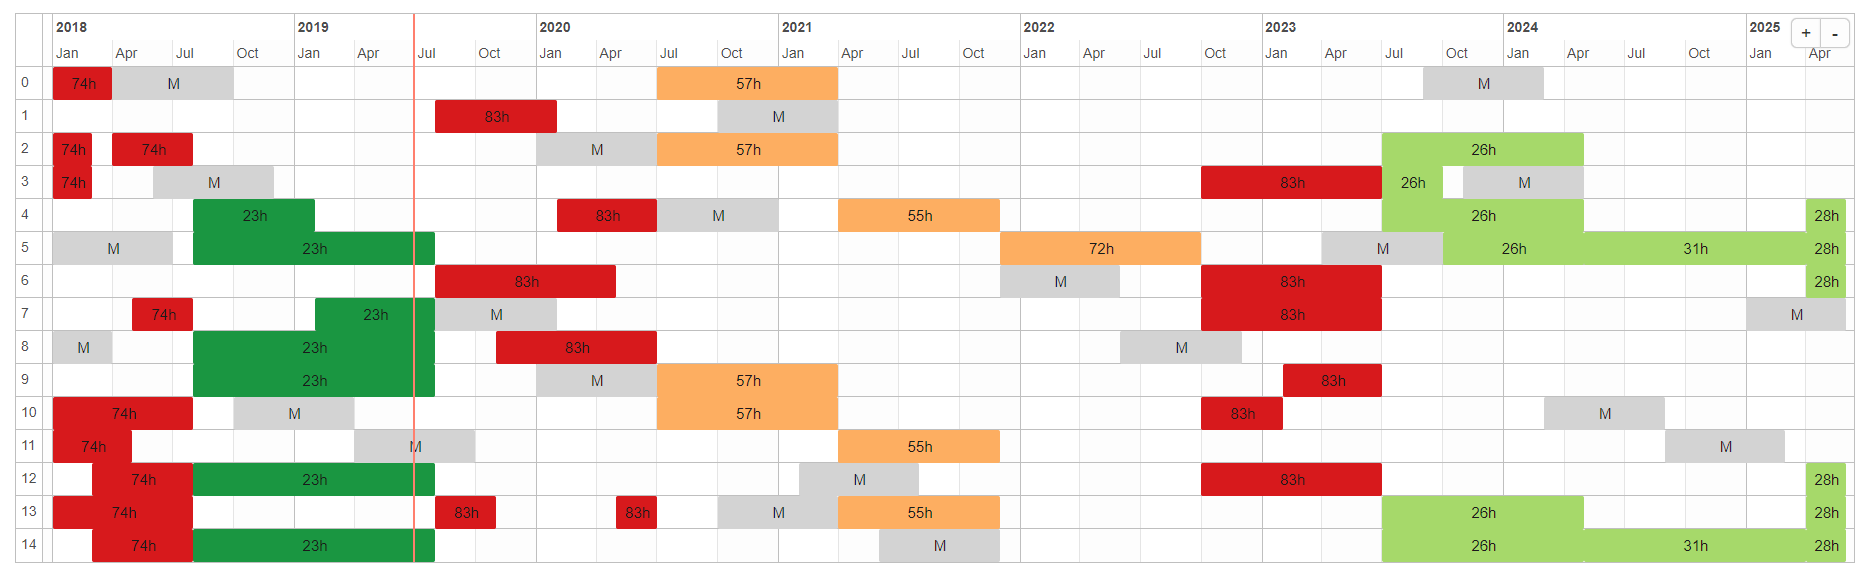
\includegraphics[width=0.7\linewidth]{calendar3}

\end{block}

\end{frame}

\begin{frame}

\begin{block}{Encoding of an MFMP solution}

\begin{align}
 a_{it} = 
  \begin{cases} 
   -1 & check \\
   0 & no\,\,assignment \\
   j & mission\,\, j \\
  \end{cases}\notag
\end{align}

Table format: a solution \(x\) is represented by a matrix
\(A = \mathbb{Z}^{I \times T}\).

Patterns: \(p \in \mathcal{P}\)

\(p = \{a_{i0}, a_{it}, a_{it+1}, ..., a_{iT}\}\)

Pattern format: a solution \(x\) is represented by a mapping
\(f: \mathcal{I} \to \mathcal{P}\).

\end{block}

\end{frame}


\miniframesoff
  \begin{frame}[noframenumbering, plain]
    \frametitle{\textbf{Outline}}
    \setbeamercovered{transparent}
  \begin{enumerate}
    \transparent{0.3}
    \item \introtitle
    \transparent{1}
    \item \textbf{\firsttitle}
    \item \secondtitle
    \item \thirdtitle
    \item \conclusiontitle
  \end{enumerate}
  \end{frame}
\miniframeson

\section[Exact methods]{\firsttitle}

\def\firsttitleF{Mixed Integer Programming model}
\def\firsttitleS{Simulated Annealing: initial solution}

\begin{frame}[t]
\frametitle{\textbf{The long term MFMP problem}}

  \begin{block}{\textbf{Basic problem}}
  \begin{columns}[c]
      \column{0.4\linewidth}

      \pause
      \begin{itemize}[<+->]
        \setbeamercolor{alerted text}{fg=black} %change the font color
        \setbeamerfont{alerted text}{series=\bfseries} %make alerted text bold
        \item \alert<2>{$j \in \mathcal{J}$ missions}.
        \item \alert<3>{$i \in \mathcal{I}$ aircraft}.
        \item \alert<4>{Maintenances}.
      \end{itemize}

      \column{0.6\linewidth}
      \only<2>{
        \begin{small}
        \begin{table}
          \centering
          \begin{tabular}{lrrrrr}
\toprule
{} &  $MT^{min}_{j}$ &  $Start_j$ &  $End_j$ &  $H_{j}$ &  $R_{j}$ \\
j &                 &            &          &          &          \\
\midrule
0 &               2 &          1 &        4 &       24 &        1 \\
1 &               2 &          5 &        7 &       34 &        3 \\
2 &               3 &          8 &       11 &       18 &        3 \\
3 &               3 &         12 &       15 &       30 &        3 \\
4 &               2 &         16 &       18 &       35 &        3 \\
5 &               2 &         19 &       20 &       25 &        1 \\
\bottomrule
\end{tabular}
        \end{table}
        \end{small}
      }
      \only<3>{
        \begin{small}
        \begin{table}
          \centering
          \begin{tabular}{lrr}
\toprule
{} &  $Rct^{Init}_i$ &  $Rft^{Init}_i$ \\
i &                 &                 \\
\midrule
0 &               7 &             120 \\
1 &              13 &             220 \\
2 &               7 &             140 \\
3 &               8 &             140 \\
4 &               6 &             160 \\
\bottomrule
\end{tabular}

        \end{table}
        \end{small}
      }
      \only<4>{
        \\
        Frequency (in time, in flight hours).\\
        Duration.\\
        Capacity.\\
      }
    \end{columns}
  \end{block} 
  

  \onslide<+->{
    \begin{block}{\textbf{More constraints}}
      Fleet-status, mission-aircraft compatibility.
    \end{block}  
  }
  \onslide<+->{
    \begin{block}{\textbf{Objectives}}
      Maximize the availability, minimize the number of checks, minimize maintenance capacity.
    \end{block}  
  }
\end{frame}

\begin{frame}[t]
\frametitle{\textbf{An example of an MFMP solution}}
  \definecolor{color2}{HTML}{D7191C}
\definecolor{color3}{HTML}{1A9641}
\definecolor{color4}{HTML}{FDAE61}
\definecolor{color5}{HTML}{A6D96A}
    \begin{ganttchart}[
    expand chart=\textwidth,
    y unit chart=0.7cm,
    hgrid,
    vgrid,
    time slot format=simple
    ]{1}{20}
    \ganttset{bar height=0.6}
    \ganttset{bar top shift=0.15}
    \gantttitlelist{1,...,20}{1} \\
\Dganttbar{0}{M}{3}{4}{bar/.append style={fill=maintColor,draw=none}}
\Dganttbar{0}{68h}{6}{7}{bar/.append style={fill=color2,draw=none}}
\Dganttbar{0}{72h}{8}{11}{bar/.append style={fill=color3,draw=none}}
\Dganttbar{0}{120h}{12}{15}{bar/.append style={fill=color4,draw=none}}
\Dganttbar{0}{M}{17}{18}{bar/.append style={fill=maintColor,draw=none}}\ganttnewline
\Dganttbar{1}{102h}{5}{7}{bar/.append style={fill=color2,draw=none}}
\Dganttbar{1}{72h}{8}{11}{bar/.append style={fill=color3,draw=none}}
\Dganttbar{1}{M}{12}{13}{bar/.append style={fill=maintColor,draw=none}}
\Dganttbar{1}{105h}{16}{18}{bar/.append style={fill=color2,draw=none}}
\Dganttbar{1}{50h}{19}{20}{bar/.append style={fill=color5,draw=none}}\ganttnewline
\Dganttbar{2}{68h}{5}{6}{bar/.append style={fill=color2,draw=none}}
\Dganttbar{2}{M}{7}{8}{bar/.append style={fill=maintColor,draw=none}}
\Dganttbar{2}{120h}{12}{15}{bar/.append style={fill=color4,draw=none}}
\Dganttbar{2}{105h}{16}{18}{bar/.append style={fill=color2,draw=none}}\ganttnewline
\Dganttbar{3}{96h}{1}{4}{bar/.append style={fill=color5,draw=none}}
\Dganttbar{3}{M}{5}{6}{bar/.append style={fill=maintColor,draw=none}}
\Dganttbar{3}{72h}{8}{11}{bar/.append style={fill=color3,draw=none}}
\Dganttbar{3}{120h}{12}{15}{bar/.append style={fill=color4,draw=none}}
\Dganttbar{3}{M}{19}{20}{bar/.append style={fill=maintColor,draw=none}}\ganttnewline
\Dganttbar{4}{M}{1}{2}{bar/.append style={fill=maintColor,draw=none}}
\Dganttbar{4}{102h}{5}{7}{bar/.append style={fill=color2,draw=none}}
\Dganttbar{4}{M}{14}{15}{bar/.append style={fill=maintColor,draw=none}}
\Dganttbar{4}{105h}{16}{18}{bar/.append style={fill=color2,draw=none}}

\node (per) [anchor=south] at ([yshift=5pt]current bounding box.north){$t$};
\node (air) [anchor=north east] at ([xshift=-5pt, yshift=-12pt]current bounding box.west){$i$};
\node (se) [anchor=north] at (current bounding box.south east){};

\end{ganttchart}

\end{frame}

  % \begin{frame}[t]
  % \frametitle{\textbf{An example of an MFMP solution}}
  %   \definecolor{color2}{HTML}{D7191C}
\definecolor{color3}{HTML}{1A9641}
\definecolor{color4}{HTML}{FDAE61}
\definecolor{color5}{HTML}{A6D96A}
% \newcommand\Dganttbar[5]{
%       \ganttbar[#5]{#1}{#3}{#4}\ganttbar[inline, bar label font=\color{white}, #5]{#2}{#3}{#4}
%     }
    \begin{ganttchart}[
    expand chart=\textwidth,
y unit chart=0.7cm,
    hgrid,
    vgrid,
    time slot format=simple
    ]{1}{20}
    \ganttset{bar height=0.6}
    \ganttset{bar top shift=0.15}
    \gantttitlelist{1,...,20}{1} \\
\Dganttbar{0}{-1}{3}{3}{bar/.append style={fill=maintColor,draw=none}}
\Dganttbar{0}{-1}{4}{4}{bar/.append style={fill=maintColor,draw=none}}
\Dganttbar{0}{2}{6}{6}{bar/.append style={fill=color2,draw=none}}
\Dganttbar{0}{2}{7}{7}{bar/.append style={fill=color2,draw=none}}
\Dganttbar{0}{3}{8}{8}{bar/.append style={fill=color3,draw=none}}
\Dganttbar{0}{3}{9}{9}{bar/.append style={fill=color3,draw=none}}
\Dganttbar{0}{3}{10}{10}{bar/.append style={fill=color3,draw=none}}
\Dganttbar{0}{3}{11}{11}{bar/.append style={fill=color3,draw=none}}
\Dganttbar{0}{4}{12}{12}{bar/.append style={fill=color4,draw=none}}
\Dganttbar{0}{4}{13}{13}{bar/.append style={fill=color4,draw=none}}
\Dganttbar{0}{4}{14}{14}{bar/.append style={fill=color4,draw=none}}
\Dganttbar{0}{4}{15}{15}{bar/.append style={fill=color4,draw=none}}
\Dganttbar{0}{-1}{17}{17}{bar/.append style={fill=maintColor,draw=none}}
\Dganttbar{0}{-1}{18}{18}{bar/.append style={fill=maintColor,draw=none}}
\Dganttbar{0}{0}{1}{1}{bar/.append style={fill=none,draw=none}}
\Dganttbar{0}{0}{2}{2}{bar/.append style={fill=none,draw=none}}
\Dganttbar{0}{0}{5}{5}{bar/.append style={fill=none,draw=none}}
\Dganttbar{0}{0}{16}{16}{bar/.append style={fill=none,draw=none}}
\Dganttbar{0}{0}{19}{19}{bar/.append style={fill=none,draw=none}}
\Dganttbar{0}{0}{20}{20}{bar/.append style={fill=none,draw=none}}\ganttnewline
\Dganttbar{1}{2}{5}{5}{bar/.append style={fill=color2,draw=none}}
\Dganttbar{1}{2}{6}{6}{bar/.append style={fill=color2,draw=none}}
\Dganttbar{1}{2}{7}{7}{bar/.append style={fill=color2,draw=none}}
\Dganttbar{1}{3}{8}{8}{bar/.append style={fill=color3,draw=none}}
\Dganttbar{1}{3}{9}{9}{bar/.append style={fill=color3,draw=none}}
\Dganttbar{1}{3}{10}{10}{bar/.append style={fill=color3,draw=none}}
\Dganttbar{1}{3}{11}{11}{bar/.append style={fill=color3,draw=none}}
\Dganttbar{1}{-1}{12}{12}{bar/.append style={fill=maintColor,draw=none}}
\Dganttbar{1}{-1}{13}{13}{bar/.append style={fill=maintColor,draw=none}}
\Dganttbar{1}{5}{16}{16}{bar/.append style={fill=color2,draw=none}}
\Dganttbar{1}{5}{17}{17}{bar/.append style={fill=color2,draw=none}}
\Dganttbar{1}{5}{18}{18}{bar/.append style={fill=color2,draw=none}}
\Dganttbar{1}{6}{19}{19}{bar/.append style={fill=color5,draw=none}}
\Dganttbar{1}{6}{20}{20}{bar/.append style={fill=color5,draw=none}}
\Dganttbar{1}{0}{1}{1}{bar/.append style={fill=none,draw=none}}
\Dganttbar{1}{0}{2}{2}{bar/.append style={fill=none,draw=none}}
\Dganttbar{1}{0}{3}{3}{bar/.append style={fill=none,draw=none}}
\Dganttbar{1}{0}{4}{4}{bar/.append style={fill=none,draw=none}}
\Dganttbar{1}{0}{14}{14}{bar/.append style={fill=none,draw=none}}
\Dganttbar{1}{0}{15}{15}{bar/.append style={fill=none,draw=none}}\ganttnewline
\Dganttbar{2}{2}{5}{5}{bar/.append style={fill=color2,draw=none}}
\Dganttbar{2}{2}{6}{6}{bar/.append style={fill=color2,draw=none}}
\Dganttbar{2}{-1}{7}{7}{bar/.append style={fill=maintColor,draw=none}}
\Dganttbar{2}{-1}{8}{8}{bar/.append style={fill=maintColor,draw=none}}
\Dganttbar{2}{4}{12}{12}{bar/.append style={fill=color4,draw=none}}
\Dganttbar{2}{4}{13}{13}{bar/.append style={fill=color4,draw=none}}
\Dganttbar{2}{4}{14}{14}{bar/.append style={fill=color4,draw=none}}
\Dganttbar{2}{4}{15}{15}{bar/.append style={fill=color4,draw=none}}
\Dganttbar{2}{5}{16}{16}{bar/.append style={fill=color2,draw=none}}
\Dganttbar{2}{5}{17}{17}{bar/.append style={fill=color2,draw=none}}
\Dganttbar{2}{5}{18}{18}{bar/.append style={fill=color2,draw=none}}
\Dganttbar{2}{0}{1}{1}{bar/.append style={fill=none,draw=none}}
\Dganttbar{2}{0}{2}{2}{bar/.append style={fill=none,draw=none}}
\Dganttbar{2}{0}{3}{3}{bar/.append style={fill=none,draw=none}}
\Dganttbar{2}{0}{4}{4}{bar/.append style={fill=none,draw=none}}
\Dganttbar{2}{0}{9}{9}{bar/.append style={fill=none,draw=none}}
\Dganttbar{2}{0}{10}{10}{bar/.append style={fill=none,draw=none}}
\Dganttbar{2}{0}{11}{11}{bar/.append style={fill=none,draw=none}}
\Dganttbar{2}{0}{19}{19}{bar/.append style={fill=none,draw=none}}
\Dganttbar{2}{0}{20}{20}{bar/.append style={fill=none,draw=none}}\ganttnewline
\Dganttbar{3}{1}{1}{1}{bar/.append style={fill=color5,draw=none}}
\Dganttbar{3}{1}{2}{2}{bar/.append style={fill=color5,draw=none}}
\Dganttbar{3}{1}{3}{3}{bar/.append style={fill=color5,draw=none}}
\Dganttbar{3}{1}{4}{4}{bar/.append style={fill=color5,draw=none}}
\Dganttbar{3}{-1}{5}{5}{bar/.append style={fill=maintColor,draw=none}}
\Dganttbar{3}{-1}{6}{6}{bar/.append style={fill=maintColor,draw=none}}
\Dganttbar{3}{3}{8}{8}{bar/.append style={fill=color3,draw=none}}
\Dganttbar{3}{3}{9}{9}{bar/.append style={fill=color3,draw=none}}
\Dganttbar{3}{3}{10}{10}{bar/.append style={fill=color3,draw=none}}
\Dganttbar{3}{3}{11}{11}{bar/.append style={fill=color3,draw=none}}
\Dganttbar{3}{4}{12}{12}{bar/.append style={fill=color4,draw=none}}
\Dganttbar{3}{4}{13}{13}{bar/.append style={fill=color4,draw=none}}
\Dganttbar{3}{4}{14}{14}{bar/.append style={fill=color4,draw=none}}
\Dganttbar{3}{4}{15}{15}{bar/.append style={fill=color4,draw=none}}
\Dganttbar{3}{-1}{19}{19}{bar/.append style={fill=maintColor,draw=none}}
\Dganttbar{3}{-1}{20}{20}{bar/.append style={fill=maintColor,draw=none}}
\Dganttbar{3}{0}{7}{7}{bar/.append style={fill=none,draw=none}}
\Dganttbar{3}{0}{16}{16}{bar/.append style={fill=none,draw=none}}
\Dganttbar{3}{0}{17}{17}{bar/.append style={fill=none,draw=none}}
\Dganttbar{3}{0}{18}{18}{bar/.append style={fill=none,draw=none}}\ganttnewline
\Dganttbar{4}{-1}{1}{1}{bar/.append style={fill=maintColor,draw=none}}
\Dganttbar{4}{-1}{2}{2}{bar/.append style={fill=maintColor,draw=none}}
\Dganttbar{4}{2}{5}{5}{bar/.append style={fill=color2,draw=none}}
\Dganttbar{4}{2}{6}{6}{bar/.append style={fill=color2,draw=none}}
\Dganttbar{4}{2}{7}{7}{bar/.append style={fill=color2,draw=none}}
\Dganttbar{4}{-1}{14}{14}{bar/.append style={fill=maintColor,draw=none}}
\Dganttbar{4}{-1}{15}{15}{bar/.append style={fill=maintColor,draw=none}}
\Dganttbar{4}{5}{16}{16}{bar/.append style={fill=color2,draw=none}}
\Dganttbar{4}{5}{17}{17}{bar/.append style={fill=color2,draw=none}}
\Dganttbar{4}{5}{18}{18}{bar/.append style={fill=color2,draw=none}}
\Dganttbar{4}{0}{3}{3}{bar/.append style={fill=none,draw=none}}
\Dganttbar{4}{0}{4}{4}{bar/.append style={fill=none,draw=none}}
\Dganttbar{4}{0}{8}{8}{bar/.append style={fill=none,draw=none}}
\Dganttbar{4}{0}{9}{9}{bar/.append style={fill=none,draw=none}}
\Dganttbar{4}{0}{10}{10}{bar/.append style={fill=none,draw=none}}
\Dganttbar{4}{0}{11}{11}{bar/.append style={fill=none,draw=none}}
\Dganttbar{4}{0}{12}{12}{bar/.append style={fill=none,draw=none}}
\Dganttbar{4}{0}{13}{13}{bar/.append style={fill=none,draw=none}}
\Dganttbar{4}{0}{19}{19}{bar/.append style={fill=none,draw=none}}
\Dganttbar{4}{0}{20}{20}{bar/.append style={fill=none,draw=none}}

% \ganttmilestone[name=start, milestone/.append style={anchor=east}]{}{0}
\node (se) [anchor=north] at (current bounding box.south east){};
\node (sw) [anchor=north] at (current bounding box.south west){};
\node (per) [anchor=south] at ([yshift=5pt]current bounding box.north){$t$};
\node (air) [anchor=north east] at ([xshift=-5pt, yshift=-12pt]current bounding box.west){$i$};
% \onslide<2->{
  \node (maint) [fill=maintColor,draw, label=left:{\tiny Check}, minimum width=0.5cm, minimum height=0.3cm, anchor=north east] at ([yshift=5pt]se.south west){\tiny\bfseries $M$};
% }
% \onslide<3->{
  \node (miss) [draw, label=left:{\tiny Mission assignment}, minimum width=0.5cm, minimum height=0.3cm, pattern=north west lines, pattern color=missionColor] at ([yshift=-12pt]maint.south){\tiny\bfseries 80h};
  \node[label=left:{\tiny Flight hours}, minimum width=0.5cm, minimum height=0.5cm] at ([yshift=-12pt]miss.south){\tiny\bfseries 80h};
% }

\onslide<2->{  
  \node[anchor=north west] at (sw.south east) {
  $\begin{aligned}
     A = \mathbb{Z}^{I \times T} = a_{it} = 
      \begin{cases} 
       -1 & check \\
       0 & no\,\,assignment \\
       j & mission\,\, j \\
      \end{cases}\notag
    \end{aligned}$
    };
}
\end{ganttchart}
  % \end{frame}

\begin{frame}
\frametitle{\textbf{Complexity analysis}}
  
  Take an instance $I$ from the MFMP problem.
  \pause
  \begin{itemize}[<+->]
    \item take out maintenances needs.
    \item no partial assignments of missions.
    \item only one aircraft needed per each mission.
    \item take out objective function: feasibility.
  \end{itemize}
  
  \begin{block}{}
  \onslide<+->{
    Becomes the NP-Complete Shift Satisfaction Personnel Task Scheduling Problem $\star$.
  }    
  \end{block}
  \begin{textblock*}{1.1\textwidth}(0.8cm, 8cm)
    \begin{flushleft}
    % $\star$
    \onslide<6->{
      \citesize $\star$ E. M. Arkin and E. B. Silverberg. Scheduling jobs with fixed start and end times. Discrete Applied Mathematics, 1987.
    }
    \end{flushleft}
  \end{textblock*}
\end{frame}

\begin{frame}
\frametitle{\textbf{Solution approaches}}
  \setbeamercovered{transparent}
  \begin{block}{\textbf{\firsttitleF}}
  \end{block}  

  \only<1>{
    \begin{block}{\textbf{\firsttitleS}}
    \end{block}  
  }
  \only<2->{
    \transparent{0.3}
    \begin{block}{\textbf{\firsttitleS}}
    \end{block}  
    \transparent{1}
  }
\end{frame}

\begin{frame}[t]
\frametitle{\textbf{\firsttitleF}}
  
  \begin{block}{Binary variables}
    \begin{tabular}{ll}
      \onslide<+->{
        $a^s_{ijt}$ &  : assignment of mission $j$ to aircraft $i$ starts in period $t$.
      }  \\
      \onslide<+->{
        $a_{ijt}$ &  :  mission $j$ assigned in period $t$ to aircraft $i$.
      }  \\
      \onslide<4->{
        $m_{it}$   & :  aircraft $i$ starts a check in period $t$.
      }
    \end{tabular}
  \end{block}

  \only<1-5>{
    \begin{adjustbox}{max totalsize={.7\textwidth}{.7\textheight},center}
      \begin{tikzpicture}
        \definecolor{color2}{HTML}{FFEDA0}
\definecolor{color3}{HTML}{ff0000}
% \definecolor{missionColor}{HTML}{00ff00}
\begin{ganttchart}[
    name = sinax,
    x unit= 0.61cm,
    % expand chart=\textwidth,
    hgrid,
    vgrid,
    milestone/.append style={fill=none, yshift=-6pt, draw=none}
]{1}{15}
    \gantttitlelist{1,...,15}{1} \\
    % \onslide<3->{
    \only<1>{
      \ganttbar[bar/.append style={pattern=north west lines, pattern color=missionColor,draw=none}, inline, bar label font=\tiny\bfseries]{}{5}{8}
      \ganttbar[bar/.append style={pattern=north west lines, pattern color=missionColor,draw=none}, inline, bar label font=\tiny\bfseries]{1}{5}{5}
    }
    \only<2>{
      \ganttbar[bar/.append style={pattern=north west lines, pattern color=missionColor,draw=none}, inline, bar label font=\tiny\bfseries]{}{5}{8}
      \ganttbar[bar/.append style={pattern=north west lines, pattern color=missionColor,draw=none}, inline, bar label font=\tiny\bfseries]{1}{5}{5}
      \ganttbar[bar/.append style={pattern=north west lines, pattern color=missionColor,draw=none}, inline, bar label font=\tiny\bfseries]{1}{6}{6}
      \ganttbar[bar/.append style={pattern=north west lines, pattern color=missionColor,draw=none}, inline, bar label font=\tiny\bfseries]{1}{7}{7}
      \ganttbar[bar/.append style={pattern=north west lines, pattern color=missionColor,draw=none}, inline, bar label font=\tiny\bfseries]{1}{8}{8}
    }
    \onslide<3->{
      \ganttbar[bar/.append style={pattern=north west lines, pattern color=missionColor,draw=none}, inline, bar label font=\tiny\bfseries]{80h}{5}{8}
    }
    \only<4>{
      \ganttbar[bar/.append style={fill=maintColor,draw=none}, inline, bar label font=\tiny\bfseries]{}{2}{3}
      \ganttbar[bar/.append style={fill=maintColor,draw=none}, inline, bar label font=\tiny\bfseries]{1}{2}{2}
    }
    \onslide<5->{
      \ganttbar[bar/.append style={fill=maintColor,draw=none}, inline, bar label font=\tiny\bfseries]{$M$}{2}{3}
    }
    \ganttmilestone[name=start, milestone/.append style={anchor=east}]{}{0}
    \ganttmilestone[name=end, milestone/.append style={anchor=east}]{}{15}
    \node (a) [anchor=north] at (current bounding box.south east){};
\end{ganttchart}

      \end{tikzpicture}  
    \end{adjustbox}
  }  
  \begin{tikzpicture}[remember picture]
\node [text width=\textwidth] {
\begin{align*}
\only<6>{&
% \overbrace{\sum_{t' \in \mathcal{T}^s_t} \sum_{i \in \mathcal{I}} m_{it'} + N_t}^{\subnode{airMaint}{}} \leq C^{\subnode{maintCap}{max}}
  \underbrace{\sum_{t' \in \mathcal{T}^s_t} \sum_{i \in \mathcal{I}} m_{it'} + N_t}_{\subnode{airMaint}{}} \leq C^{max}_{\subnode{maintCap}{}}
      & t \in \mathcal{T}\\  
}
\onslide<7->{& 
  \sum_{t' \in \mathcal{T}^s_t} \sum_{i \in \mathcal{I}} m_{it'} + N_t \leq C^{max}
      & t \in \mathcal{T}\\
}
% min assignments:
\only<7>{& 
  \underbrace{\sum_{i \in \mathcal{I}_j} a_{ijt}}_{\subnode{airMission}{}} \geq R_{\subnode{missionNeed}{j}}
      & j \in \mathcal{J}, t \in \mathcal{T}_j \\
} 
\onslide<8->{& 
  \sum_{i \in \mathcal{I}_j} a_{ijt} \geq R_j
      & j \in \mathcal{J}, t \in \mathcal{T}_j \\
} 
% just doing one thing at any given time:
\only<8>{&
   \underbrace{\sum_{t' \in \mathcal{T}^s_t} m_{it'} + \sum_{j \in \mathcal{J}_t \cap \mathcal{O}_i} a_{ijt}}_{\subnode{airNum}{}} \leq 1 
      & t \in \mathcal{T}, i \in \mathcal{I}
      }
\end{align*}
      };
\node (ref) at (-4,-1.5) {};
\node (ref2) at (2,-1.5) {};
\only<6>{
  \node [expla] (demand) at (ref) {Number of aircraft in maintenance in period $t$};
  \draw[bend right=20,->] (demand) to (airMaint.south);
  \node [expla] (capacity) at (ref2) {Maintenance capacity};
  \draw[bend left=20,->] (capacity) to (maintCap.east);
}
\only<7>{
  \node [expla] (assigned) at (ref) {Number of aircraft assigned to mission $j$ in period $t$};
  \draw[bend right=20,->] (assigned.north) to (airMission.south);
  \node [expla] (needs) at (ref2) {Mission needs of mission $j$};
  \draw[bend left=20,->] (needs.west) to (missionNeed.south);
}
\only<8>{
  \node [expla] (numberText) at ([yshift=-5pt]ref2.south) {Assignments of aircraft $i$ in period $t$};
  \draw[bend left=20,->] (numberText.south west) to (airNum.south);
}

\end{tikzpicture}
\end{frame}

\begin{frame}[t]
\frametitle{\textbf{\firsttitleF: Flight hours rule}}
  \begin{block}{Continuous variables}
    \begin{tabular}{ll}
      \onslide<1->{
        $u_{it}$ &: flight hours by aircraft $i$ during period $t$.
      }  \\
      \onslide<3->{
        $rft_{it}$ &: remaining flight hours for aircraft $i$ during period $t$.
      }  \\
    \end{tabular}
  \end{block}

  \onslide<1->{
    \begin{adjustbox}{max totalsize={.7\textwidth}{.7\textheight},center}
      \begin{tikzpicture}
        \definecolor{color2}{HTML}{FFEDA0}
\definecolor{color3}{HTML}{ff0000}
% \definecolor{missionColor}{HTML}{00ff00}
\begin{ganttchart}[
    name = sinax,
    x unit= 0.61cm,
    % expand chart=\textwidth,
    hgrid,
    vgrid,
    milestone/.append style={fill=none, yshift=-6pt, draw=none}
]{1}{15}
    \gantttitlelist{1,...,15}{1} \\

    % \onslide<2>{
    % \ganttbar[bar/.append style={pattern=north west lines, pattern color=missionColor,draw=none}, inline, bar label font=\tiny\bfseries]{80h}{5}{8}
    % \ganttbar[bar/.append style={fill=maintColor,draw=none}, inline, bar label font=\tiny\bfseries]{$M$}{2}{3}
    % }

    \onslide<1-2>{
      \ganttbar[bar/.append style={pattern=north west lines, pattern color=missionColor,draw=none}, inline, bar label font=\tiny\bfseries]{20h}{5}{5}
      \ganttbar[bar/.append style={pattern=north west lines, pattern color=missionColor,draw=none}, inline, bar label font=\tiny\bfseries]{20h}{6}{6}
      \ganttbar[bar/.append style={pattern=north west lines, pattern color=missionColor,draw=none}, inline, bar label font=\tiny\bfseries]{20h}{7}{7}
      \ganttbar[bar/.append style={pattern=north west lines, pattern color=missionColor,draw=none}, inline, bar label font=\tiny\bfseries]{20h}{8}{8}
      \ganttbar[bar/.append style={draw=none}, inline, bar label font=\tiny\bfseries]{0h}{1}{1}
      \ganttbar[bar/.append style={draw=none}, inline, bar label font=\tiny\bfseries]{0h}{4}{4}
      \ganttbar[bar/.append style={draw=none}, inline, bar label font=\tiny\bfseries]{0h}{9}{9}
      \ganttbar[bar/.append style={draw=none}, inline, bar label font=\tiny\bfseries]{0h}{10}{10}
      \ganttbar[bar/.append style={draw=none}, inline, bar label font=\tiny\bfseries]{0h}{11}{11}
      \ganttbar[bar/.append style={draw=none}, inline, bar label font=\tiny\bfseries]{0h}{12}{12}
      \ganttbar[bar/.append style={draw=none}, inline, bar label font=\tiny\bfseries]{0h}{13}{13}
      \ganttbar[bar/.append style={draw=none}, inline, bar label font=\tiny\bfseries]{0h}{14}{14}
      \ganttbar[bar/.append style={draw=none}, inline, bar label font=\tiny\bfseries]{0h}{15}{15}
      \ganttbar[bar/.append style={fill=maintColor,draw=none}, inline, bar label font=\tiny\bfseries]{0h}{2}{2}
      \ganttbar[bar/.append style={fill=maintColor,draw=none}, inline, bar label font=\tiny\bfseries]{0h}{3}{3}
    }
    \onslide<3->{
      \ganttbar[bar/.append style={pattern=north west lines, pattern color=missionColor,draw=none}, inline, bar label font=\tiny\bfseries]{80h}{5}{5}
      \ganttbar[bar/.append style={pattern=north west lines, pattern color=missionColor,draw=none}, inline, bar label font=\tiny\bfseries]{60h}{6}{6}
      \ganttbar[bar/.append style={pattern=north west lines, pattern color=missionColor,draw=none}, inline, bar label font=\tiny\bfseries]{40h}{7}{7}
      \ganttbar[bar/.append style={pattern=north west lines, pattern color=missionColor,draw=none}, inline, bar label font=\tiny\bfseries]{20h}{8}{8}
      % \ganttbar[bar/.append style={draw=none}, inline, bar label font=\tiny\bfseries]{$Rft^{Init}$}{1}{1}
      \ganttbar[bar/.append style={draw=none}, inline, bar label font=\tiny\bfseries]{50h}{1}{1}
      \ganttbar[bar/.append style={draw=none}, inline, bar label font=\tiny\bfseries]{100h}{4}{4}
      \ganttbar[bar/.append style={draw=none}, inline, bar label font=\tiny\bfseries]{20h}{9}{9}
      \ganttbar[bar/.append style={draw=none}, inline, bar label font=\tiny\bfseries]{20h}{10}{10}
      \ganttbar[bar/.append style={draw=none}, inline, bar label font=\tiny\bfseries]{20h}{11}{11}
      \ganttbar[bar/.append style={draw=none}, inline, bar label font=\tiny\bfseries]{20h}{12}{12}
      \ganttbar[bar/.append style={draw=none}, inline, bar label font=\tiny\bfseries]{20h}{13}{13}
      \ganttbar[bar/.append style={draw=none}, inline, bar label font=\tiny\bfseries]{20h}{14}{14}
      \ganttbar[bar/.append style={draw=none}, inline, bar label font=\tiny\bfseries]{20h}{15}{15}
      % \ganttbar[bar/.append style={fill=maintColor,draw=none}, inline, bar label font=\tiny\bfseries]{$H^{max}$}{2}{2}
      \ganttbar[bar/.append style={fill=maintColor,draw=none}, inline, bar label font=\tiny\bfseries]{100h}{2}{2}
      \ganttbar[bar/.append style={fill=maintColor,draw=none}, inline, bar label font=\tiny\bfseries]{100h}{3}{3}
    }
    % \node (b) [anchor=north] at ([yshift=-0.4cm]current bounding box.south west){};
    % \node (per) [anchor=south] at ([yshift=5pt]current bounding box.north){$t$};
    % \node (air) [anchor=north east] at ([xshift=-5pt, yshift=-12pt]current bounding box.west){$i$};
    % \onslide<2->{
    % \node (maint) [fill=maintColor,draw, label=left:{\tiny Check}, minimum width=0.5cm, minimum height=0.15cm, anchor=west] at ([yshift=3pt,xshift=1cm]b.south){};
    % }
    % \onslide<3->{
    % \node (miss) [draw, label=left:{\tiny Mission assignment}, minimum width=0.5cm, minimum height=0.15cm, pattern=north west lines, pattern color=missionColor, anchor=west] at ([xshift=3cm]maint.east){};
      % \node[label=left:{\tiny Flight hours}, minimum width=0.5cm, minimum height=0.5cm, anchor=west] at ([xshift=2cm]miss.east){\tiny\bfseries 80h};
    % }

    % \ganttmilestone[name=start, milestone/.append style={anchor=east}]{}{0}
    % \ganttmilestone[name=end, milestone/.append style={anchor=east}]{}{15}
    % \node (a) [anchor=north] at (current bounding box.south east){};
\end{ganttchart}

      \end{tikzpicture}  
    \end{adjustbox}
  }

  \begin{align*}
    \only<2>{
      & u_{it} \geq \sum_{j \in \mathcal{J}_t \cap \mathcal{O}_i} a_{ijt} H_j 
          & t =1, ..., \mathcal{T}, i \in \mathcal{I} \\
      & u_{it} \geq U^{min} (1 - \sum_{t' \in \mathcal{T}^s_t} m_{it'})
          & t =1, ..., \mathcal{T}, i \in \mathcal{I} \\
      & u_{it} \in [0, \max_j{\{H_j\}}]
            & t =1, ..., \mathcal{T}, i \in \mathcal{I} \\
    }
    \only<4->{
      & rft_{i0} = Rft^{Init}_i
             & i \in \mathcal{I}\\
      & rft_{it} \leq rft_{i(t-1)} + H^M m_{it} - u_{it}
          & t =1, ..., \mathcal{T}, i \in \mathcal{I} \\
      & rft_{it} \geq H^M m_{it'}
              & t \in \mathcal{T}, t' \in \mathcal{T}^s_t, i \in \mathcal{I}\\ 
      & rft_{it} \in [0,H^M]
              & t \in \mathcal{T}, i \in \mathcal{I}
    }
  \end{align*}
\end{frame}

\begin{frame}
\frametitle{\textbf{Solution approaches}}
  \setbeamercovered{transparent}
  \transparent{0.3}
  \begin{block}{\textbf{\firsttitleF}}
  \end{block}  
  \transparent{1}

  \begin{block}{\textbf{\firsttitleS}}
  \end{block}  
\end{frame}

\begin{frame}
\frametitle{\textbf{\firsttitleS}}
  % \pause
  \definecolor{color2}{HTML}{D7191C}
\definecolor{color3}{HTML}{1A9641}
\definecolor{color4}{HTML}{FDAE61}
\definecolor{color5}{HTML}{A6D96A}
    \begin{ganttchart}[
    expand chart=\textwidth,
    y unit chart=0.7cm,
    hgrid,
    vgrid,
    time slot format=simple
    ]{1}{20}
    \ganttset{bar height=0.6}
    \ganttset{bar top shift=0.15}
    \gantttitlelist{1,...,20}{1} \\
    \onslide<1->{
      \Dganttbar{0}{M}{3}{4}{bar/.append style={fill=maintColor,draw=none}}
      \Dganttbar{0}{M}{17}{18}{bar/.append style={fill=maintColor,draw=none}}
    }
    \onslide<2->{
      \Dganttbar{0}{68h}{6}{7}{bar/.append style={fill=color2,draw=none}}
      \Dganttbar{0}{72h}{8}{11}{bar/.append style={fill=color3,draw=none}}
      \Dganttbar{0}{120h}{12}{15}{bar/.append style={fill=color4,draw=none}}
    }
    \ganttnewline
    \onslide<1->{
      \Dganttbar{1}{M}{12}{13}{bar/.append style={fill=maintColor,draw=none}}
    }
    \onslide<2->{
      \Dganttbar{1}{102h}{5}{7}{bar/.append style={fill=color2,draw=none}}
      \Dganttbar{1}{72h}{8}{11}{bar/.append style={fill=color3,draw=none}}
      \Dganttbar{1}{105h}{16}{18}{bar/.append style={fill=color2,draw=none}}
      \Dganttbar{1}{50h}{19}{20}{bar/.append style={fill=color5,draw=none}}
    }
    \ganttnewline
    \onslide<1->{
      \Dganttbar{2}{M}{7}{8}{bar/.append style={fill=maintColor,draw=none}}
    }
    \onslide<2->{
    \Dganttbar{2}{68h}{5}{6}{bar/.append style={fill=color2,draw=none}}
    \Dganttbar{2}{120h}{12}{15}{bar/.append style={fill=color4,draw=none}}
    \Dganttbar{2}{105h}{16}{18}{bar/.append style={fill=color2,draw=none}}
    }
    \ganttnewline
    \onslide<1-2,6>{
    \Dganttbar{3}{M}{5}{6}{bar/.append style={fill=maintColor,draw=none}}
    \Dganttbar{3}{M}{19}{20}{bar/.append style={fill=maintColor,draw=none}}
    }
    \onslide<2,6>{
    \Dganttbar{3}{96h}{1}{4}{bar/.append style={fill=color5,draw=none}}
    \Dganttbar{3}{72h}{8}{11}{bar/.append style={fill=color3,draw=none}}
    \Dganttbar{3}{120h}{12}{15}{bar/.append style={fill=color4,draw=none}}
    }
    \onslide<4-5>{
    \Dganttbar{3}{M}{9}{10}{bar/.append style={fill=maintColor,draw=none}}
    }
    \onslide<5>{
    \Dganttbar{3}{96h}{1}{4}{bar/.append style={fill=color5,draw=none}}
    \Dganttbar{3}{120h}{12}{15}{bar/.append style={fill=color4,draw=none}}
    }
    \ganttnewline
    \onslide<1->{
    \Dganttbar{4}{M}{1}{2}{bar/.append style={fill=maintColor,draw=none}}
    \Dganttbar{4}{M}{14}{15}{bar/.append style={fill=maintColor,draw=none}}
    }
    \onslide<2->{
    \Dganttbar{4}{102h}{5}{7}{bar/.append style={fill=color2,draw=none}}
    \Dganttbar{4}{105h}{16}{18}{bar/.append style={fill=color2,draw=none}}
    }

    \node (per) [anchor=south] at ([yshift=5pt]current bounding box.north){$t$};
    \node (air) [anchor=north east] at ([xshift=-5pt, yshift=-12pt]current bounding box.west){$i$};
    \node (se) [anchor=north] at (current bounding box.south east){};

    \node (maint) [fill=maintColor,draw, label=left:{\tiny Check}, minimum width=0.5cm, minimum height=0.3cm, anchor=north east] at ([yshift=5pt]se.south west){\tiny\bfseries $M$};
    \node (miss) [draw, label=left:{\tiny Mission assignment}, minimum width=0.5cm, minimum height=0.3cm, fill=missionColor] at ([yshift=-12pt]maint.south){\tiny\bfseries 80h};
    \node[label=left:{\tiny Flight hours}, minimum width=0.5cm, minimum height=0.5cm] at ([yshift=-12pt]miss.south){\tiny\bfseries 80h};

\end{ganttchart}
  
\end{frame}

\begin{frame}
\frametitle{\textbf{Experiments}}

  \textbf{Instance simulator}.
  \pause
  \begin{itemize}
    \item Several parameters and configurations.
    \begin{itemize}
      \item Fleet sizes ($|\mathcal{I}|$): 15 (base), 30, 45, 60.
      \item Planning horizons ($|\mathcal{T}|$): 90 (base), 120, 140.
    \end{itemize}
    \item Number of instances per dataset: 50.  
    \item Resolution: CPLEX with a time limit of 1 hour.
  \end{itemize}
\end{frame}

\begin{frame}
\frametitle{\textbf{Results}}

  \begin{itemize}[<+->]
    \item Small gaps overall.
    \item Solution times highly sensible on the size of the instance.
  \end{itemize}
  
  \only<1>{
    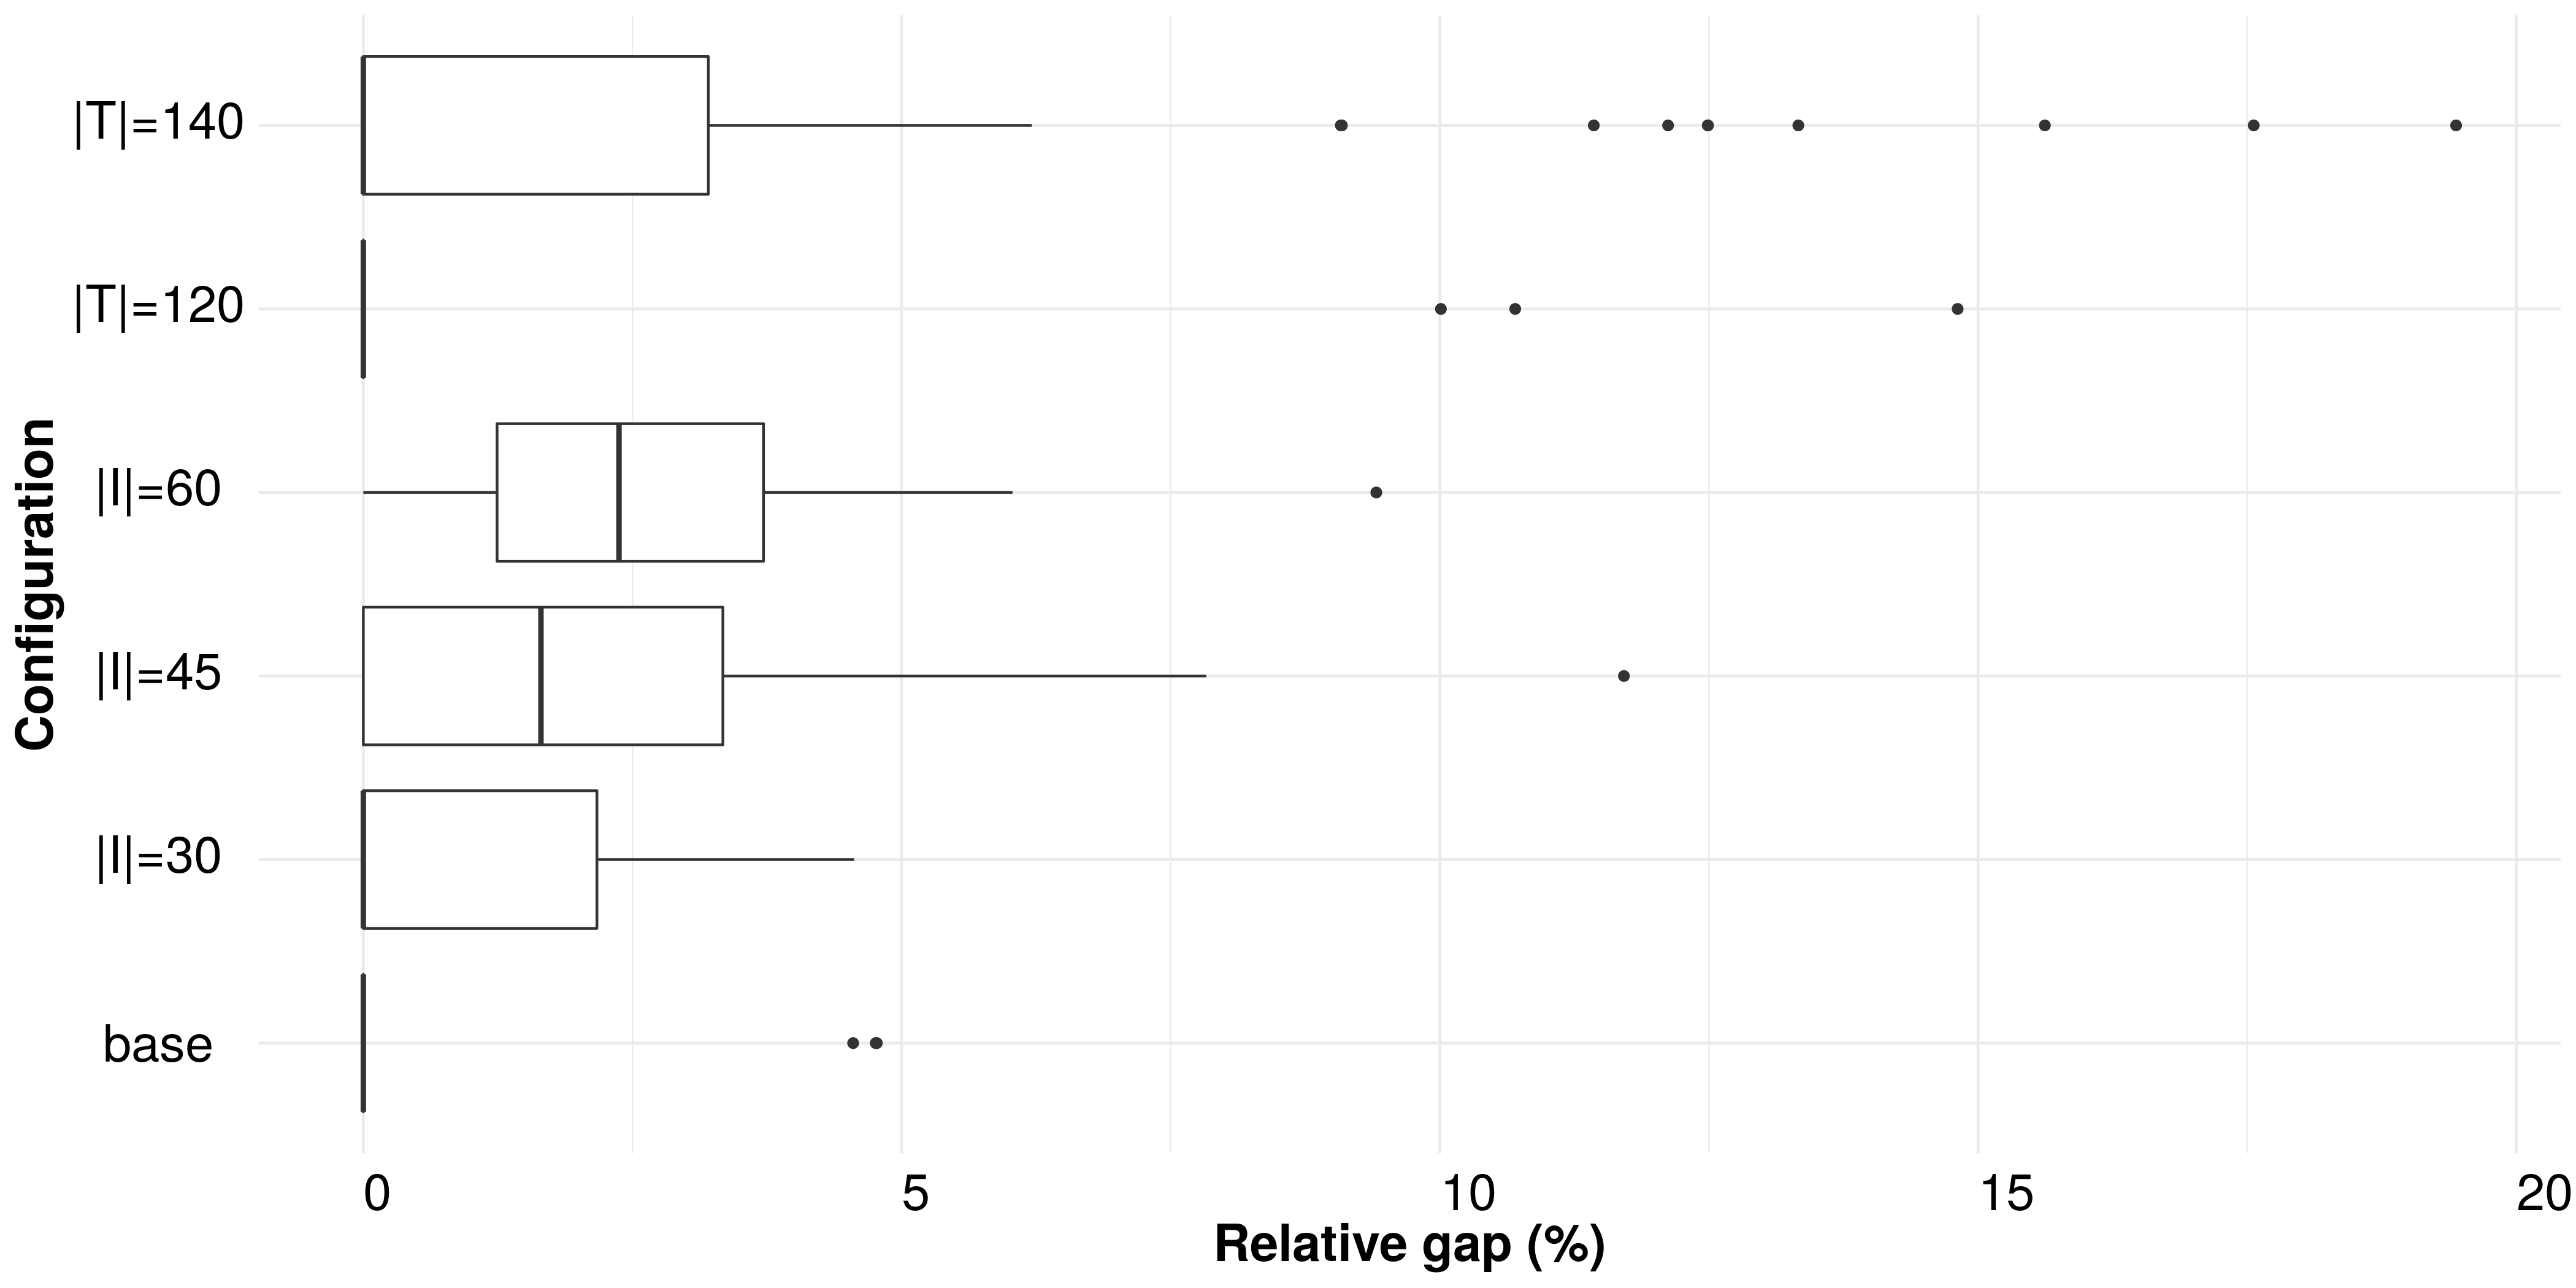
\includegraphics[width=\linewidth]{images/clust1_20190322_gaps.png}
  }
  \only<2>{
    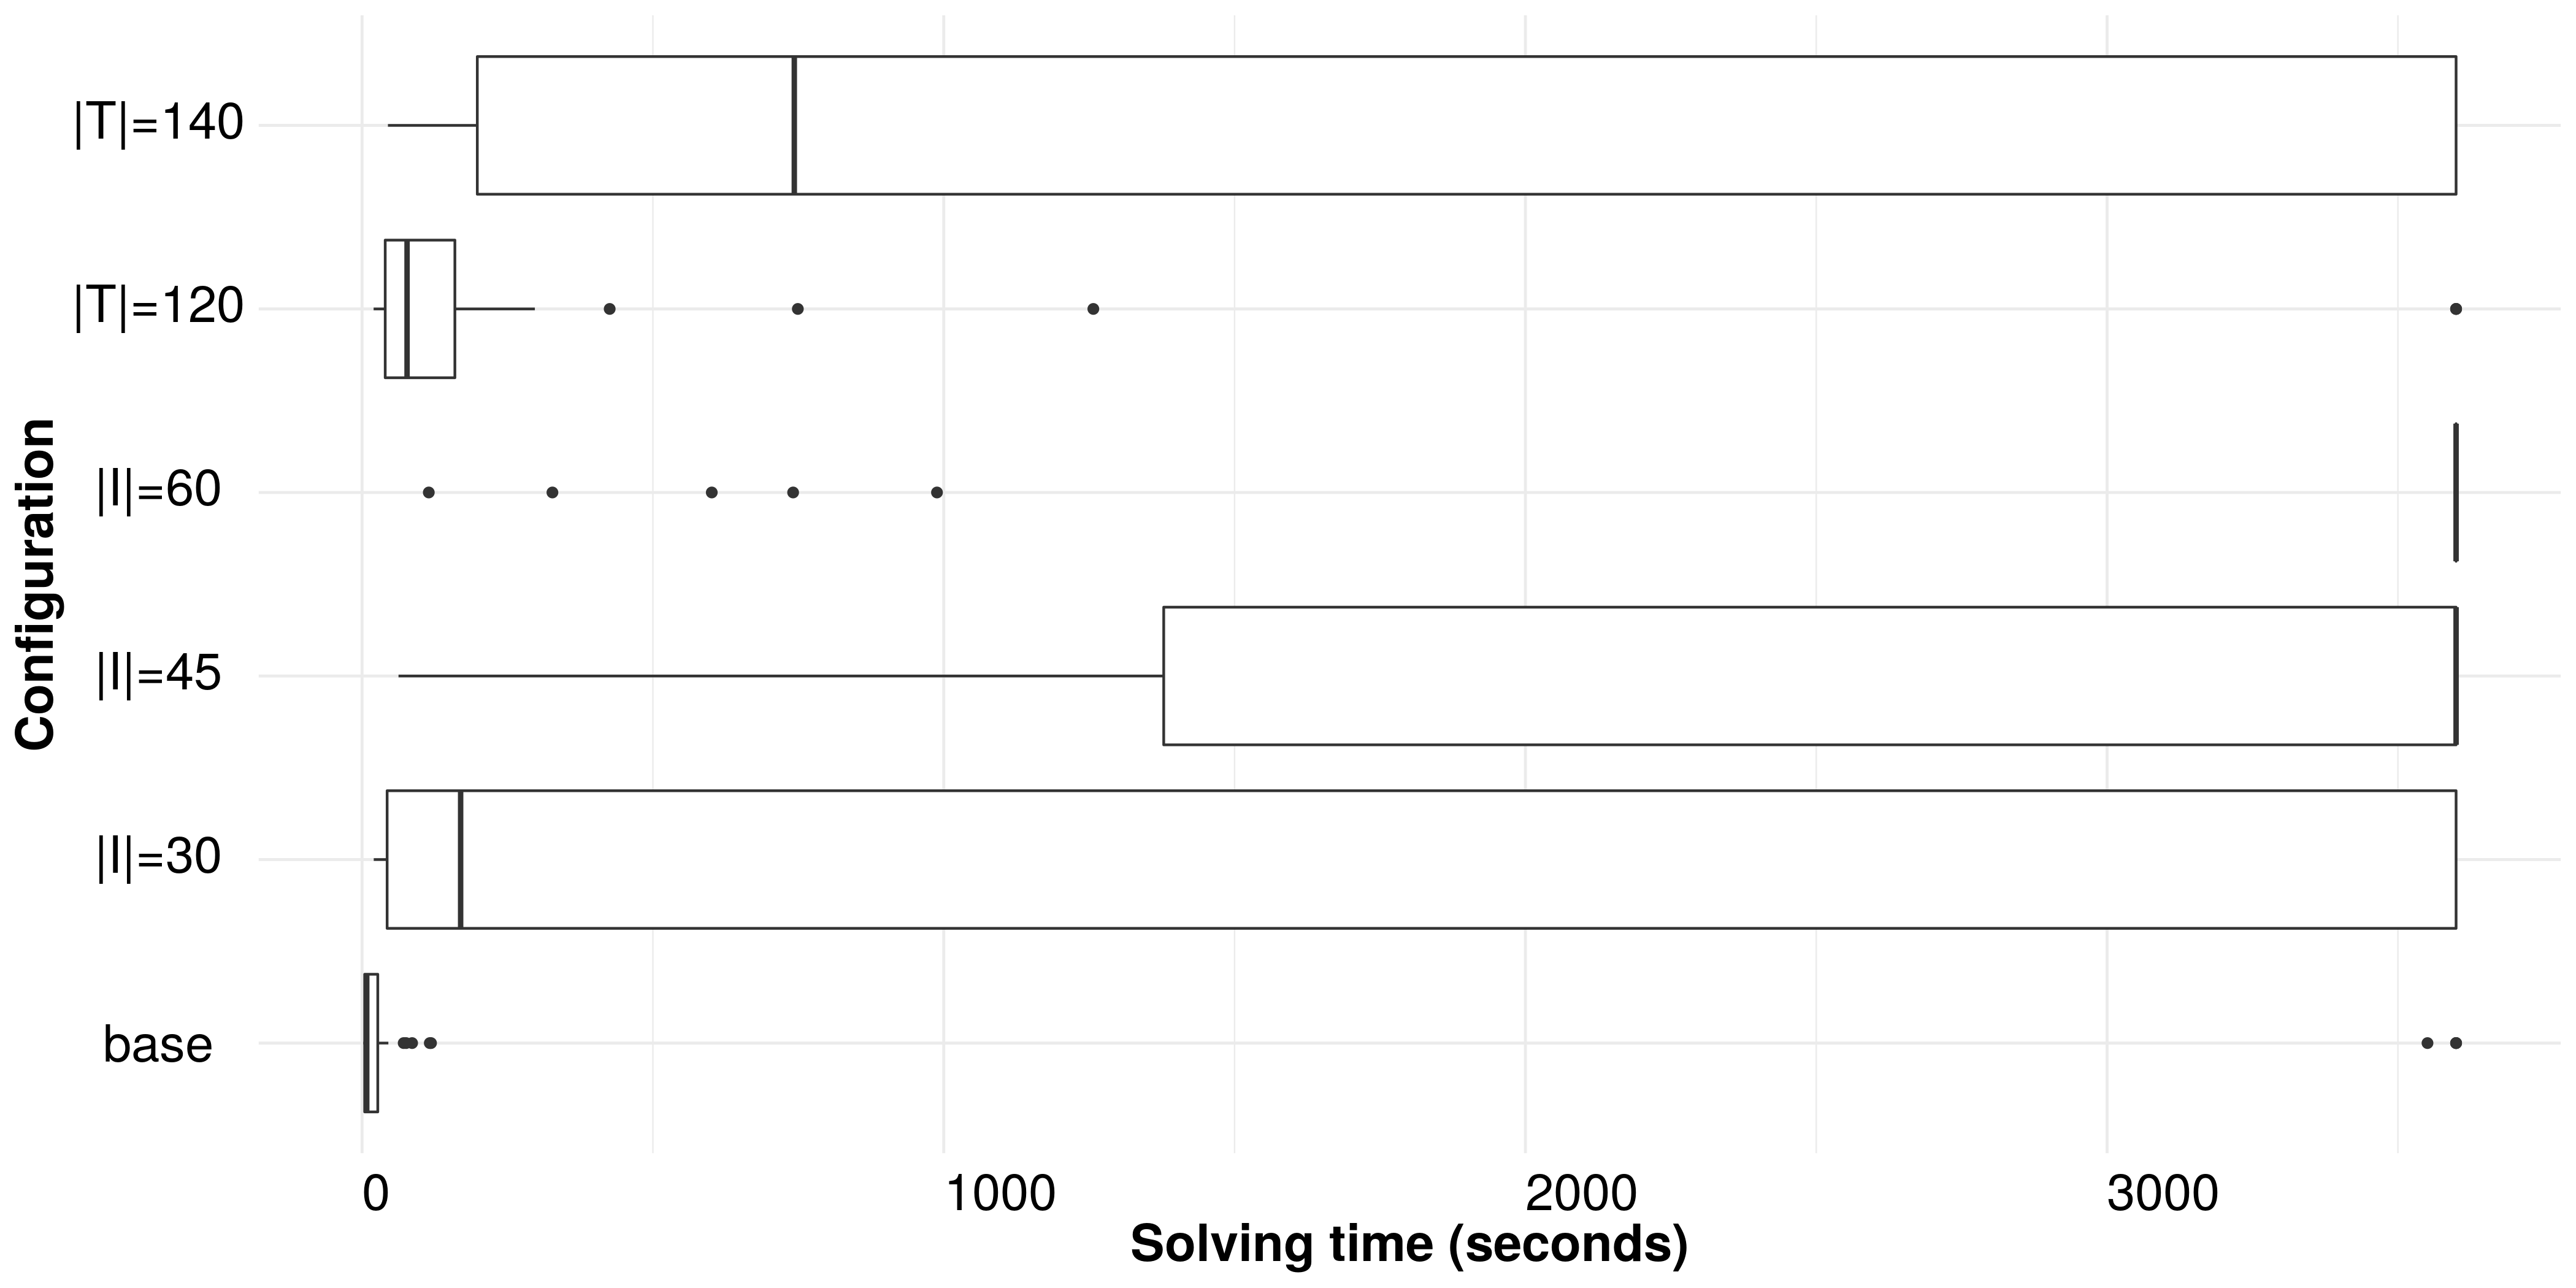
\includegraphics[width=\linewidth]{images/clust1_20190322_times.png}
  }
\end{frame}

\begin{frame}
\frametitle{\textbf{Preliminary conclusions}}
  % \begin{block}{}
    \begin{itemize}[<+->]
    \item \textbf{The long term MFMP problem is presented}
      along with a complexity analysis and a configurable instance generator.
    \item \textbf{Two solving techniques are tested}:
      a MIP model and a Simulated Annealing approach.  
    \item \textbf{Improvements are needed} 
      to reduce the model's sensibility to the size of instances.
    \end{itemize}
  % \end{block}  
  % \pause
  % \begin{block}{\textbf{Perspectives}}
  %   \begin{itemize}
  %     \item \textbf{Extend the problem} to include some additional secondary constraints.        
      
        
  %   \end{itemize}
  % \end{block}
  % \pause
  \onslide<+->{
    \textbf{Submission:} Franco Peschiera, Olga Battaïa, Alain Haït, Nicolas Dupin. Long term planning of military aircraft flight and maintenance operations. Annals of Operations Research.
  }
\end{frame}


\miniframesoff
  \begin{frame}[noframenumbering, plain]
    \frametitle{\textbf{Outline}}
    \setbeamercovered{transparent}
  \begin{enumerate}
    \transparent{0.3}
    \item \introtitle
    \item \firsttitle
    \transparent{1}
    \item \textbf{\secondtitle}
    \item \thirdtitle
    \item \conclusiontitle
  \end{enumerate}
  \end{frame}
\miniframeson

\section{\secondtitle}

\def\secondtitleF{Predicting learned-cuts}
\def\secondtitleS{Applying learned-cuts to the MFMP}


\begin{frame}
\frametitle{\textbf{Contents}}
  \setbeamercovered{transparent}
  \begin{block}{\textbf{\secondtitleF}}
  \end{block}  

  \only<1>{
    \begin{block}{\textbf{\secondtitleS}}
    \end{block}  
  }
  \only<2->{
    \transparent{0.3}
    \begin{block}{\textbf{\secondtitleS}}
    \end{block}  
    \transparent{1}
  }

\end{frame}

\begin{frame}[t]
\frametitle{\textbf{Predicting learned-cuts}}
  \pause
  \begin{tabular}{ll}
  \onslide<+->{
    \textbf{Optimization problem} & $y^{*}(x) :\equiv arg \,\,\min_{y \in \mathcal{Y}(x)} C(x,y)$
    } \\
  \onslide<+->{
      \textbf{Solution features} & $G(y) = \{g_n(y) \,\, \forall n \in \mathcal{N}\}$
  } \\
  \onslide<+->{
      \textbf{Input features} & $H(x) = \{h_m(x) \,\, \forall m \in \mathcal{M}\}$ 
  }\\ 
  \onslide<6->{
      \textbf{Training for optimal} & $G(y^*(x)) \approx \hat{G}(x) = f(H(x))$
  } \\
  \end{tabular}

  \only<2>{
   \begin{adjustbox}{max totalsize={.5\textwidth}{.5\textheight},center}
      \DrawSolution{none}{none}{0}
   \end{adjustbox}
  }
  \only<3-4>{
   \begin{adjustbox}{max totalsize={.5\textwidth}{.5\textheight},center}
      \DrawSolution{gy}{none}{0}
   \end{adjustbox}
  }
  \only<5->{
   \begin{adjustbox}{max totalsize={.5\textwidth}{.5\textheight},center}
      \DrawSolution{gyoptim}{none}{0}
   \end{adjustbox}
  }
  % \only<6->{
  %   \Put(0,20){
  %    \begin{adjustbox}{max totalsize={.5\textwidth}{.5\textheight},center}
  %       \DrawSolution{none}{none}{0}
  %    \end{adjustbox}
  %   }
  %   \Put(0,40){
  %    \begin{adjustbox}{max totalsize={.5\textwidth}{.5\textheight},center}
  %       \DrawSolution{none}{none}{0}
  %    \end{adjustbox}
  %   }
  %   \Put(0,60){
  %    \begin{adjustbox}{max totalsize={.5\textwidth}{.5\textheight},center}
  %       \DrawSolution{none}{none}{0}
  %    \end{adjustbox}
  %   }
  % }

\end{frame}

\begin{frame}[t]
\frametitle{\textbf{Applying learned-cuts}}

  \begin{tabular}{ll}
  \onslide<2->{
    \textbf{We predict the optimal features} & $\hat{G}(x) = \hat{g}_n(x) \,\, \forall n \in \mathcal{N}$
    } \\
  \onslide<3->{
      \textbf{We predict the optimal ``zone''} & $\mathcal{Y}^\prime(x) = \{y \in \mathcal{Y} \mid  \hat{G}(x) = G(y) \}$
  } \\
  \onslide<4->{
      \textbf{We solve the predicted model} & $\hat{y}^{*}(x) :\equiv arg \,\,\min_{y \in \mathcal{Y}^\prime(x)} C(x,y)$ 
  }\\ 
  \onslide<5->{
      \textbf{With some (hopefully small) loss} & $C(x,\hat{y}^{*}(x)) \approx  C(x,y^{*}(x))$
  } \\
  \end{tabular}

  \only<1>{
   \begin{adjustbox}{max totalsize={.5\textwidth}{.5\textheight},center}
      \DrawSolution{none}{none}{0}
   \end{adjustbox}
  }
  \only<2>{
   \begin{adjustbox}{max totalsize={.5\textwidth}{.5\textheight},center}
      \DrawSolution{ghat}{none}{0}
   \end{adjustbox}
  }
  \only<3>{
   \begin{adjustbox}{max totalsize={.5\textwidth}{.5\textheight},center}
      \DrawSolution{ghat}{north west lines}{0}
   \end{adjustbox}
   }
  \only<4>{
   \begin{adjustbox}{max totalsize={.5\textwidth}{.5\textheight},center}
      \DrawSolution{ghat}{north west lines}{1}
   \end{adjustbox}
   }
  \onslide<5->{
   \begin{adjustbox}{max totalsize={.5\textwidth}{.5\textheight},center}
      \DrawSolution{ghat}{north west lines}{2}
   \end{adjustbox}
   }
\end{frame}

% \begin{frame}
% \frametitle{\textbf{Optimality of learned-cuts}}

%   \begin{columns}[c]
%     \column{0.6\linewidth}
%     \textbf{With some (hopefully small) loss :}
%     \column{0.4\linewidth}
%     \begin{equation*}
%       C(x,\hat{y}^{*}(x)) \approx  C(x,y^{*}(x))
%     \end{equation*}
%   \end{columns}
%   \only<1>{
%    \begin{adjustbox}{max totalsize={.5\textwidth}{.5\textheight},center}
%       \DrawSolution{ghat}{north west lines}{1}
%    \end{adjustbox}
%    }
%   \only<2->{
%    \begin{adjustbox}{max totalsize={.5\textwidth}{.5\textheight},center}
%       \DrawSolution{ghat}{north west lines}{2}
%    \end{adjustbox}
%    }
%    % TODO: legend
% \end{frame}

\begin{frame}
\frametitle{\textbf{Motivation}}

  \pause
  \begin{enumerate}[<+->]
  \item
    \textbf{Performance}: a smaller model is easier to solve.
  \item
    \textbf{User feedback}: direct feedback about the solution without
    needing to solve any model.
  \end{enumerate}
\end{frame}

\begin{frame}
\frametitle{\textbf{Contents}}
  \setbeamercovered{transparent}
  \transparent{0.3}
  \begin{block}{\textbf{\secondtitleF}}
  \end{block}  
  \transparent{1}

  \begin{block}{\textbf{\secondtitleS}}
  \end{block}  
\end{frame}


\begin{frame}[t]
\frametitle{\textbf{New formulation}}

% TODO: legend, aircraft i, period t, M= check
  
  \begin{tabular}{ll}
    \onslide<2->{$a_{ijtt'}$ & : aircraft $i$ is in mission $j$ between $t$ and $t'$.}  \\
    \onslide<3->{$m_{ip}$ &: aircraft $i$ uses check pattern $p$.} \\
  \end{tabular}

  \onslide<5->{
    \begin{align}
      & \sum_{(j, t, t') \in \mathcal{J}\mathcal{T}\mathcal{T}_{ic}} a_{ijtt'} H^\prime_{jtt'} + U^{\prime}_{tc} \leq H^{M} + bigM (1 - m_{ip}) & \notag \\
      & \hspace{200px}  i \in \mathcal{I}, p \in \mathcal{P}, c \in \mathcal{C}_p \notag
    \end{align}
  }

  \only<1>{
    \DrawGantt{0}{0}{0}
  }
  \only<2>{
    % missions
    \DrawGantt{0}{1}{0}
  }
  \only<3>{
    % maintenances and missions
    \DrawGantt{2}{1}{0}
  }
  \only<4->{
    % maints, missions and cycles
    \DrawGantt{2}{1}{cycle}
  }
\end{frame}

\begin{frame}
\frametitle{\textbf{Solution feature: distance between maintenances}}

  For each aircraft $i$: $D_i(y) \in [E^{min},E^{max}] \,\, \forall y \in \mathcal{Y}(x)$. \\
  \only<+->{
    \DrawGantt{2}{0}{distance}
  }
  \onslide<+->{
    Solution feature: $g_1(y) = \mu_{t'-t} = \frac {\sum_{i \in \mathcal{I}} D_i(y)}{I}$. \\
  }

  % \only<4->{
  %   Distribution of $\mu^*_{t'-t}$: \\
  % 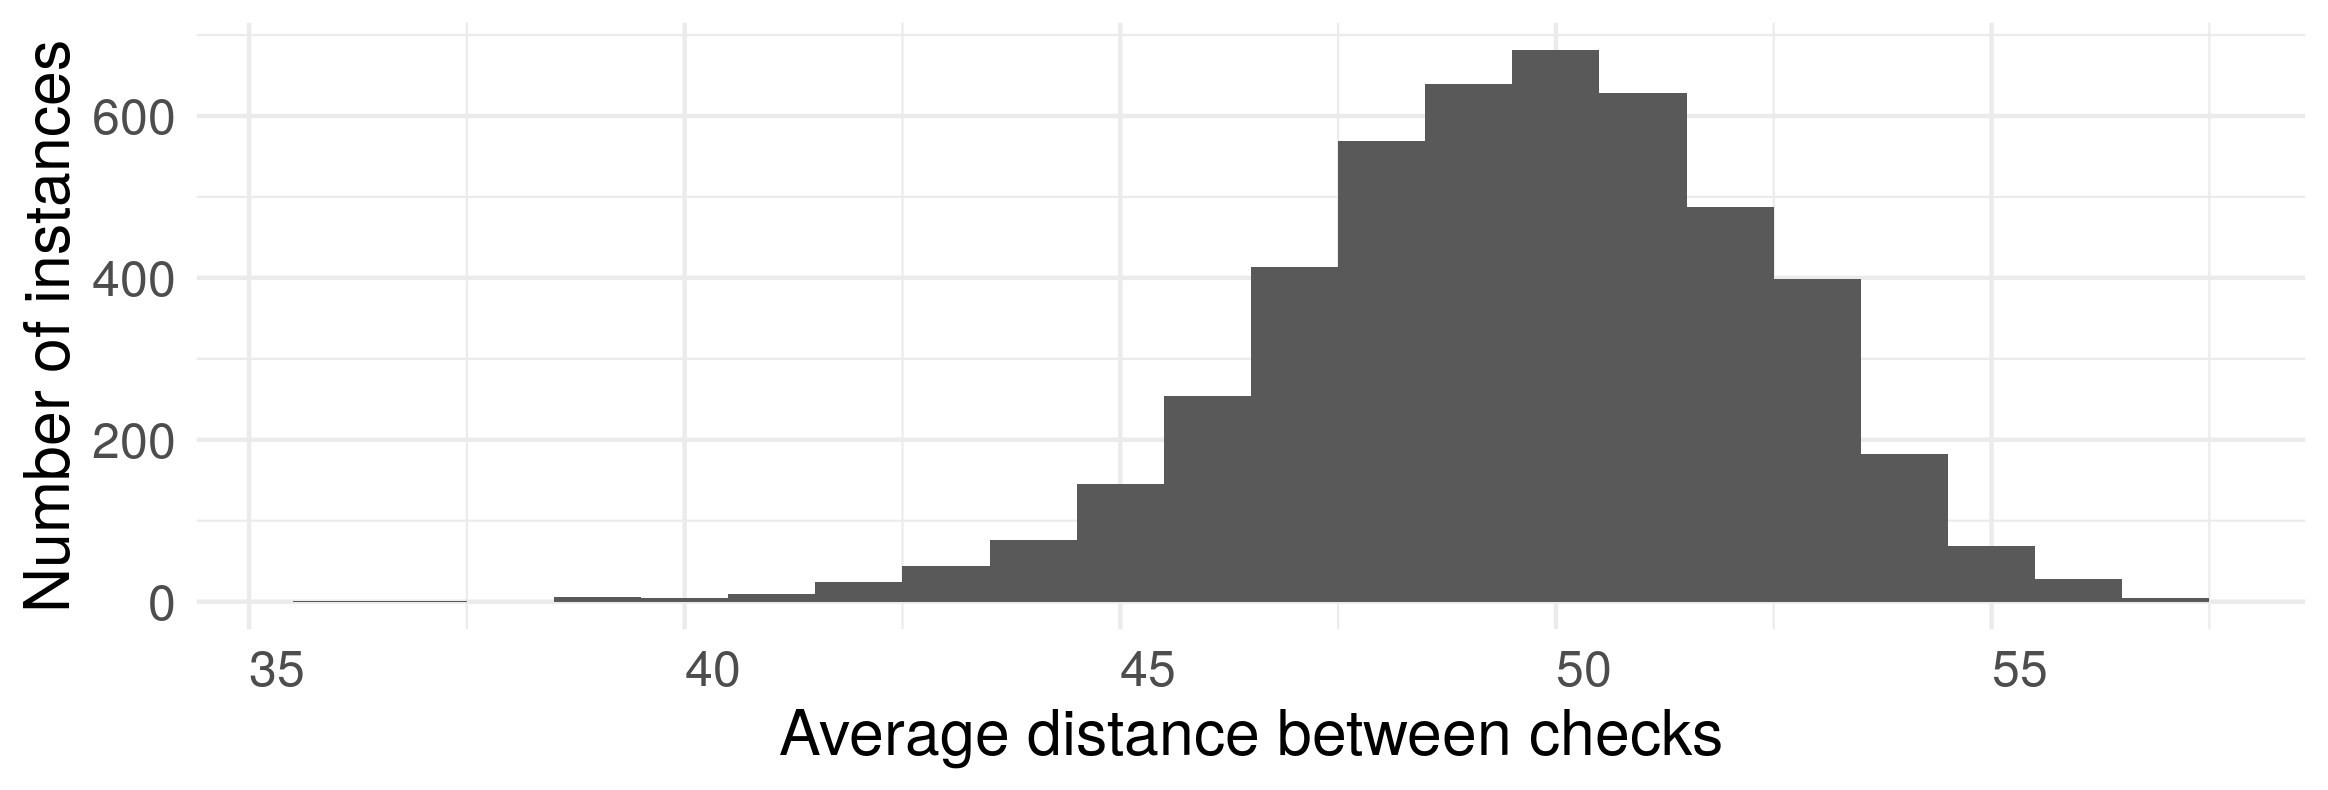
\includegraphics[height=0.3\linewidth]{images/distribution_mean_distances_IT000125_20190716}
  % }

\end{frame}

\begin{frame}
\frametitle{\textbf{Input features}}

  \onslide<1->{  
    \begin{block}{\textbf{Mission related}}
      Max, average, variance of flight hours per period. Median period.
    \end{block}
  }
  \onslide<2->{  
    \begin{block}{\textbf{Fleet related}}
      Sum of initial status (rft).
    \end{block}
  }
  \onslide<3->{  
    \begin{block}{\textbf{Compatibility related}}
      Sum of all special mission flight hours.
    \end{block}
  }
\end{frame}

\begin{frame}
\frametitle{\textbf{Forecasting technique}}

  \onslide<1->{  
    \begin{block}{\textbf{Quantile regressions}}
      Upper bound and lower bound at 10\% and 90\%.
      \begin{equation*}
        \mu_{t'-t} \to [\hat{\mu}_{t'-t}^{lb}, \hat{\mu}_{t'-t}^{ub}]
     \end{equation*}
    \end{block}
  }
  \onslide<2->{  
  \begin{block}{\textbf{Training / test set}}
    of 5000 small instances solved to optimal and splitted: 70/30.
  \end{block}
  }

  % TODO: add prediction results
  % TODO: add prediction example
\end{frame}

\begin{frame}
\frametitle{\textbf{Applying learned-cuts}}

  \begin{block}{\textbf{Pattern filtering:}}
    \begin{equation*}
      D_{ip} \in [\hat{\mu}_{t'-t}^{lb} - tol, \hat{\mu}_{t'-t}^{ub} + tol] \rightarrow p \in \mathcal{P}_i 
    \end{equation*}
  \end{block}
  % TODO: add example
  \pause

  \begin{block}{\textbf{Pattern recycling:} with probabiliy $\alpha$}
    \begin{equation*}
      D_{ip} \notin [\hat{\mu}_{t'-t}^{lb} - tol, \hat{\mu}_{t'-t}^{ub} + tol] \land P(\alpha)  \rightarrow p \in \mathcal{P}_i 
    \end{equation*}
  \end{block}
\end{frame}

\begin{frame}
\frametitle{\textbf{Experiments}}
  \begin{itemize}

  \item Number of instances: medium (1000), large (1000) and very large
    (1000).
  \item Time limit at 3600 seconds.
  \item We seeded instance generation for better comparison.
  \item CPLEX running 1 thread.
  \end{itemize}

  Largest instances have 60 aircraft, 90 periods.
\end{frame}

\begin{frame}
\frametitle{\textbf{Results: performance}}

  % TODO: change colors
  % TODO: bigger picture
  \begin{itemize}[<+->]
    \item More solutions.
    \item Faster solutions.
  \end{itemize}

  \only<1>{
    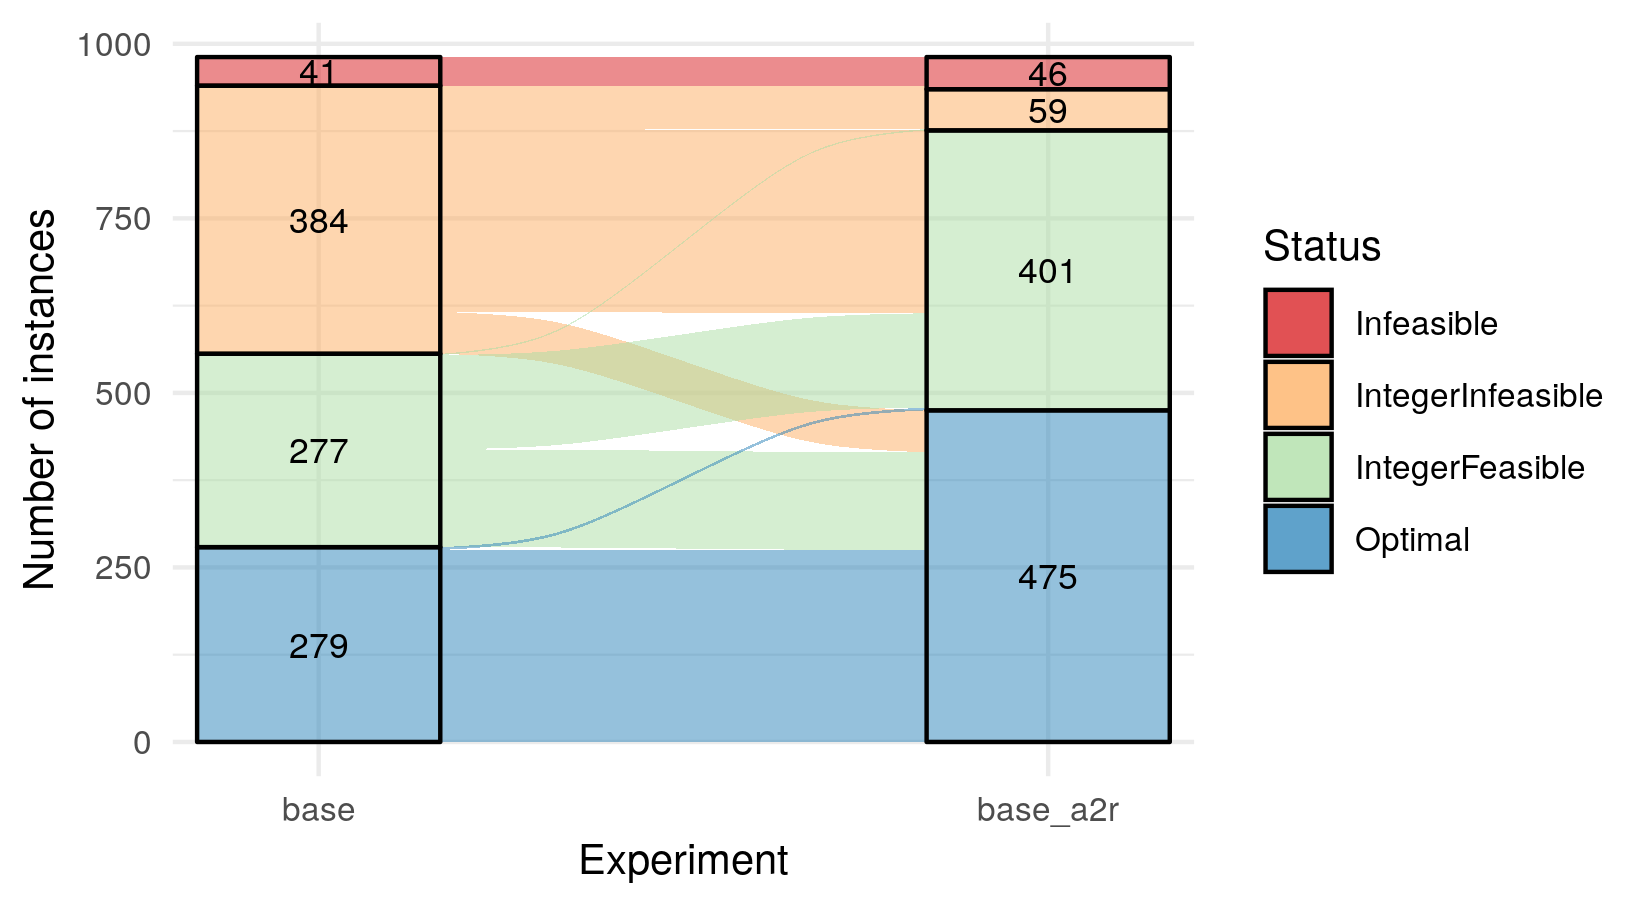
\includegraphics[width=0.8\linewidth]{images/transitions_base_2tasks.png}
  }
  \only<2>{
  % TODO: add one line at a time.
  % TODO: lines thicker and lines, not points
  % TODO: Time to solve instance (seconds)
    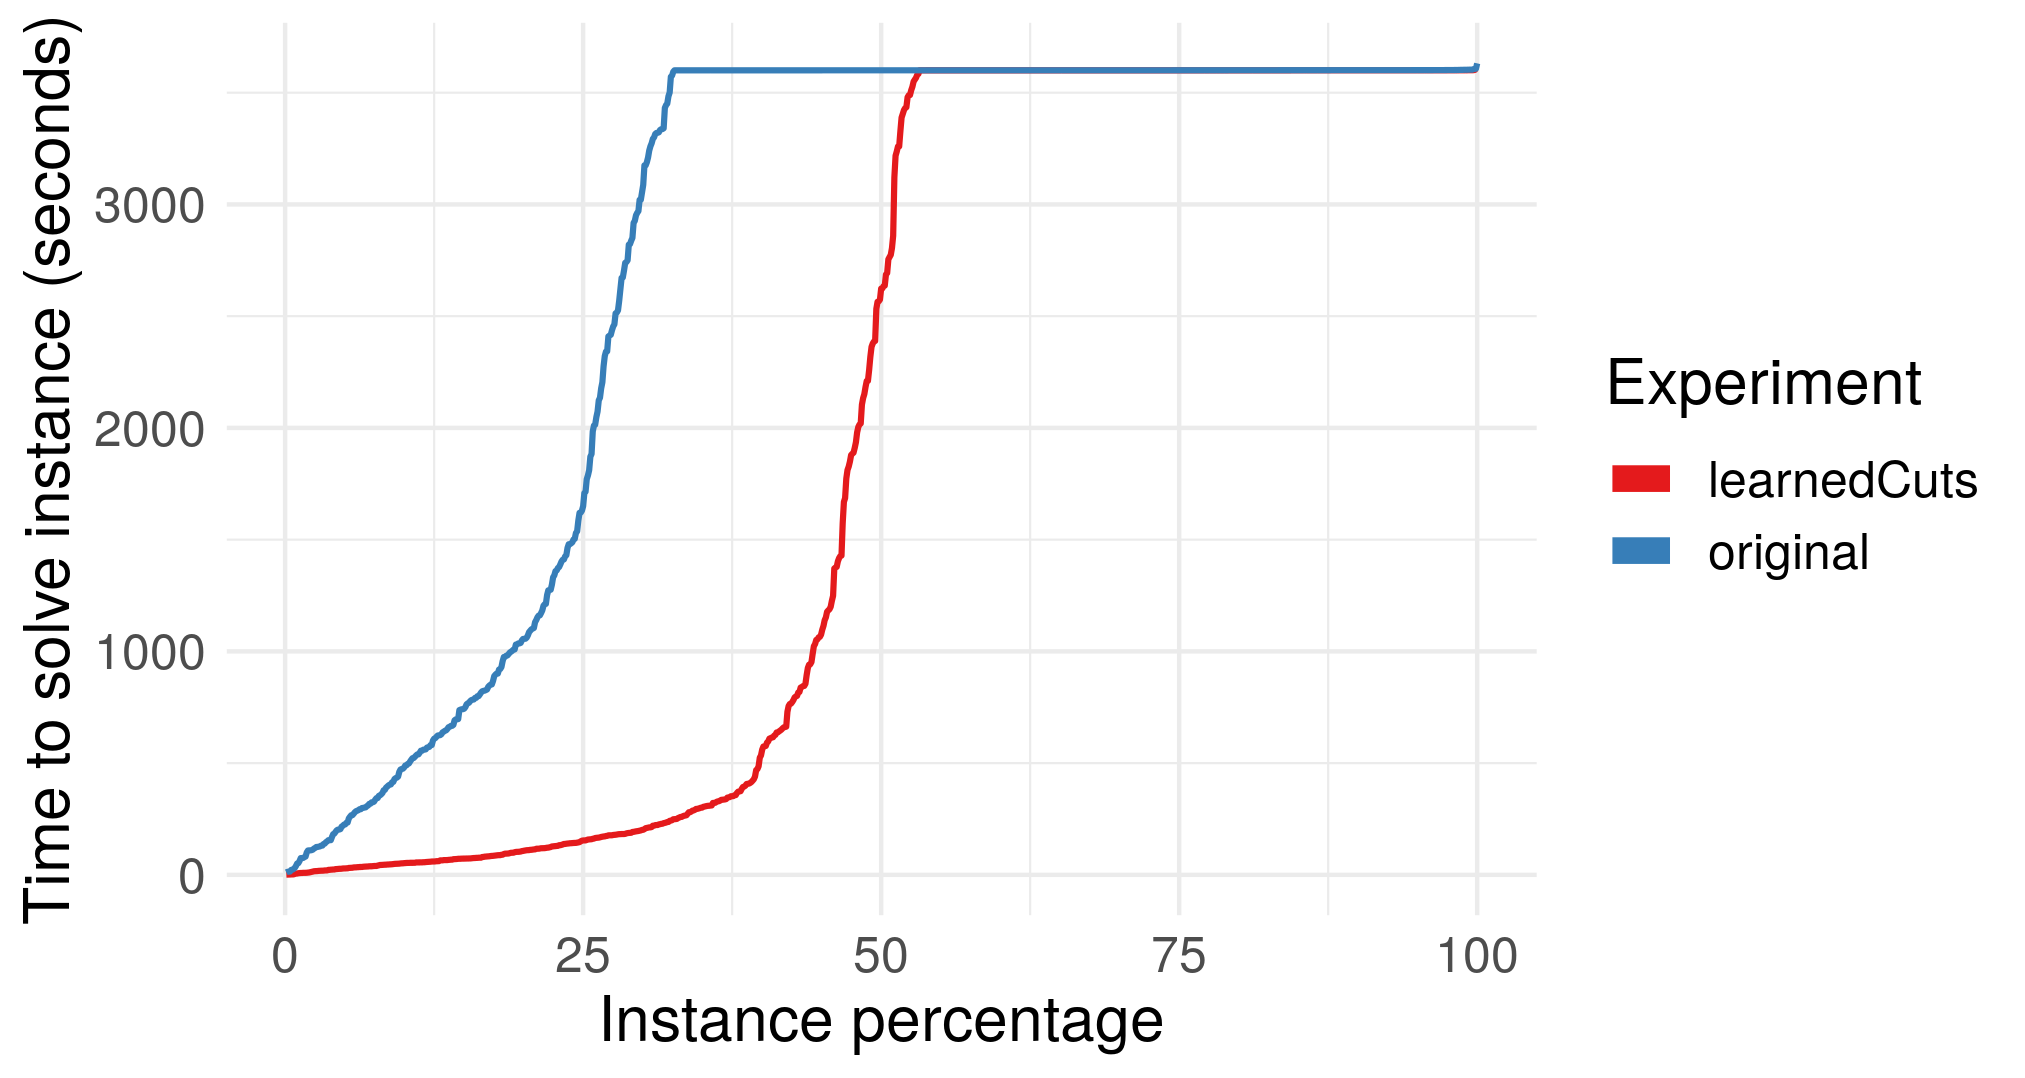
\includegraphics[width=0.8\linewidth]{images/time_performance_ordered_2tasks.png}
  }
\end{frame}

\begin{frame}
\frametitle{\textbf{Results: optimality}}
  
  \begin{itemize}[<+->]
    \item $\le$ 7\% loss of optimality for $\ge$ 95\%.
    \item better predictions can improve this.
  \end{itemize}

  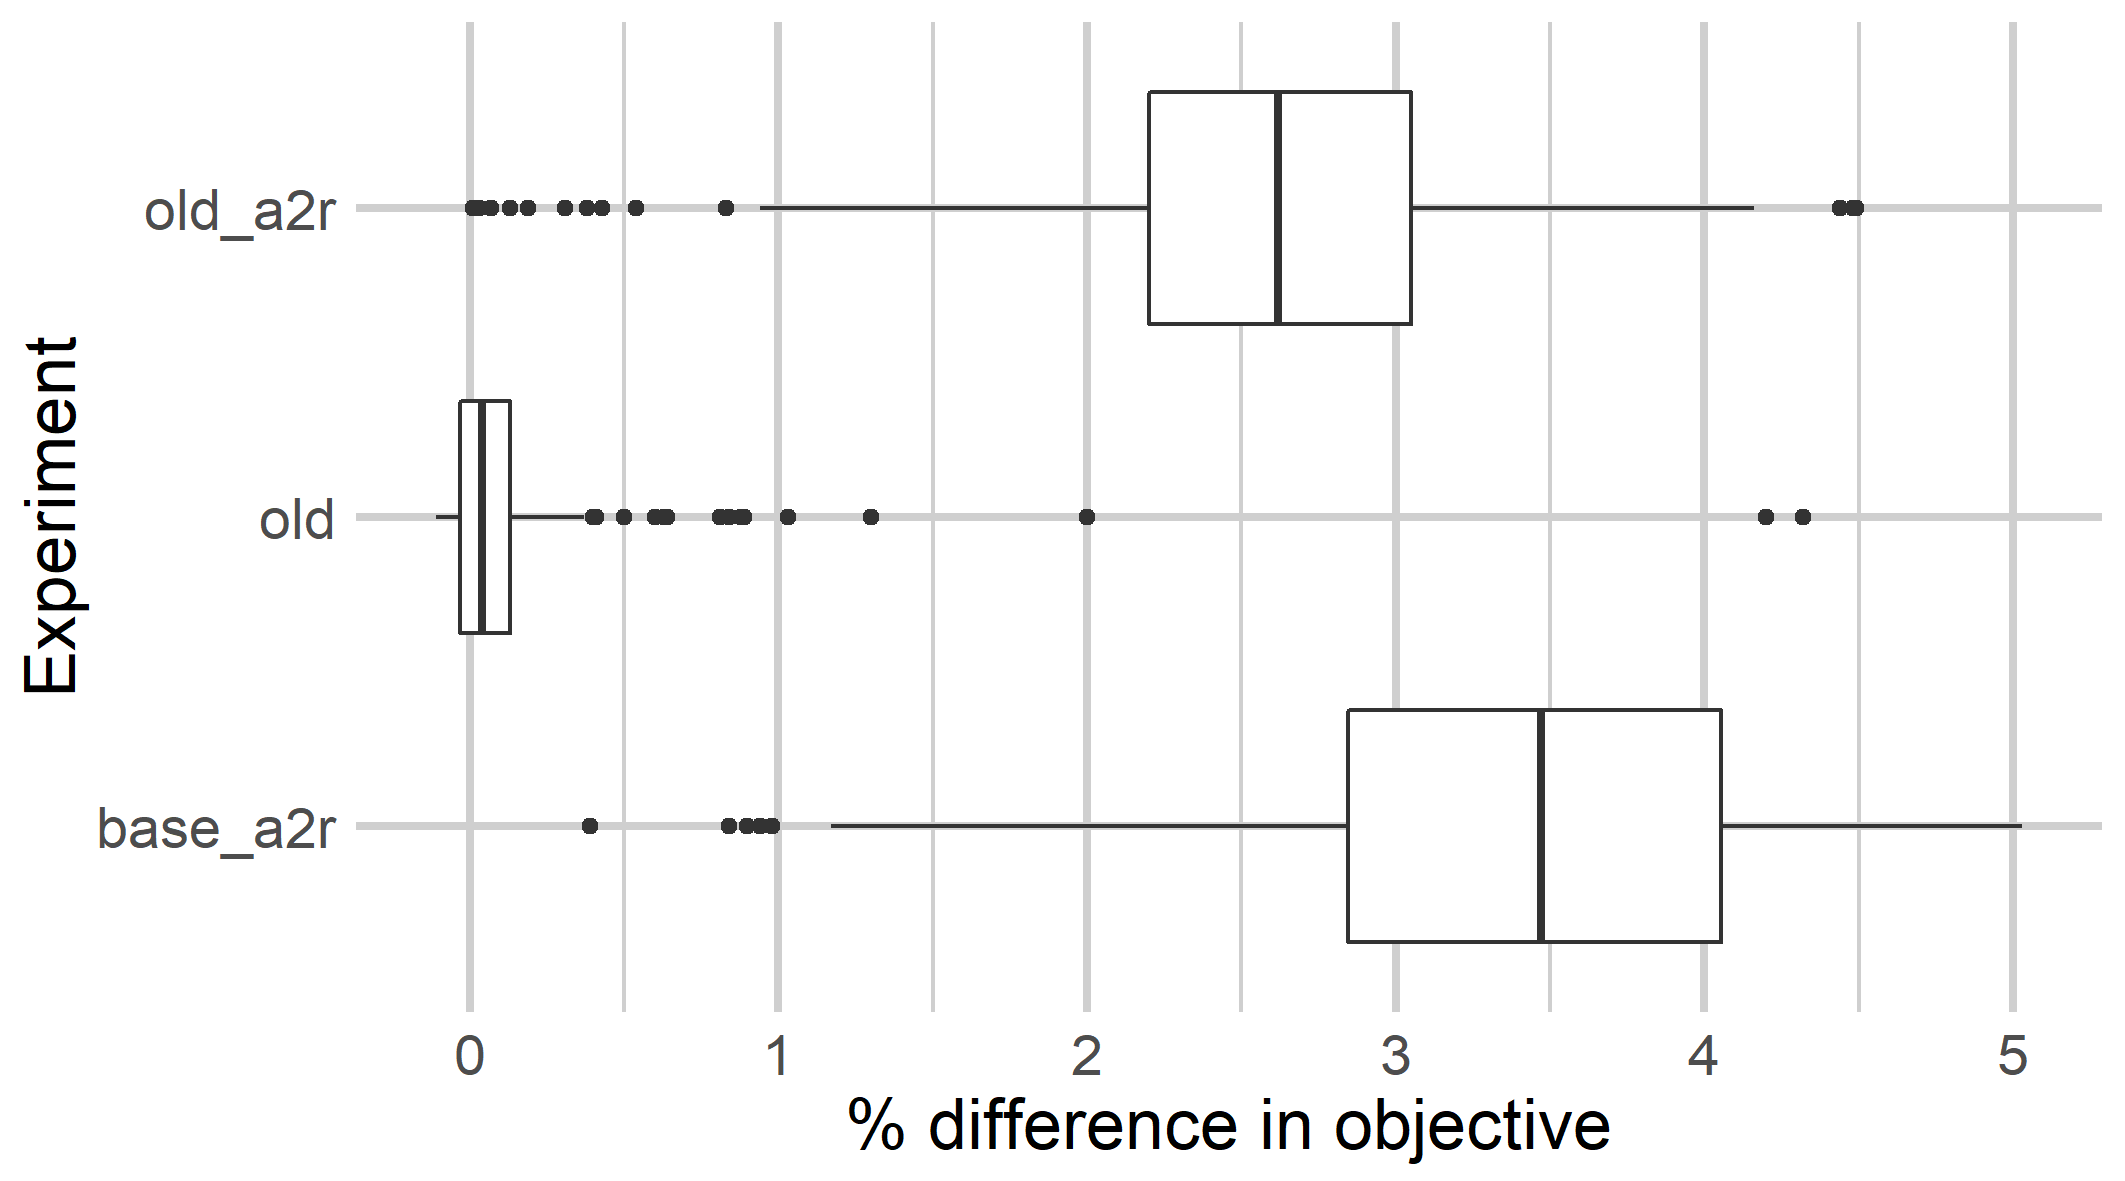
\includegraphics[width=0.8\linewidth]{images/quality_degradation_2tasks}

\end{frame}

\begin{frame}
\frametitle{\textbf{Preliminary conclusions}}
  \pause
  % TODO: check phrases
  \begin{block}{\textbf{Conclusions}}
    \begin{itemize}[<+->]
    \item \textbf{Supervised learning for optimization}
      provides good heuristic solutions.
    \item \textbf{MFMP application}
      shows the benefits of such an approach.
    \end{itemize}
  \end{block}  
  \pause
  \begin{block}{\textbf{Perspectives}}
    \begin{itemize}[<+->]
      \item \textbf{Generalize methodology} 
        to obtain a probability distribution for patterns, automatize feature extraction.
      \item \textbf{Combine it with other techniques} 
        to warm-start Column Generation, use a graph-based dynamic pattern generation.
    \end{itemize}
  \end{block}  
\end{frame}

\miniframesoff
  \begin{frame}[noframenumbering, plain]
    \frametitle{\textbf{Outline}}
    \setbeamercovered{transparent}
  \begin{enumerate}
    \transparent{0.3}
    \item \introtitle
    \item \firsttitle
    \item \secondtitle
    \transparent{1}
    \item \textbf{\thirdtitle}
    \item \conclusiontitle
  \end{enumerate}
  \end{frame}
\miniframeson

\section{\thirdtitle}

\begin{frame}
\frametitle{\textbf{Patterns}}
  \begin{tabular}{p{5mm}p{90mm}}
    $b_{ip}$ &: aircraft $i$ uses check pattern $p$. \\
  \end{tabular}

  % TODO: this image
  % j and M => legend
  \DrawGantt{2}{2}{0}

\end{frame}

\begin{frame}
\frametitle{\textbf{Pattern representation}}
  % TODO: legend aircraft i, t, etc.
  % TODO: animation to explain a node, legend
  % TOOD: redo a simpler graph


\def\mydata{1, 2, 3, 4, 5, 6, 7, 8}

\foreach \x in \mydata
{
\pgfmathtruncatemacro\z{\x-1}
% \z{}
 \only<\x>{
    \begin{adjustbox}{max totalsize={\textwidth}{\textheight},center}
      \DrawGraph{\z}
   \end{adjustbox}
 }
}
  \only<1-2>{
  \DrawGantt{0}{0}{0}
  }
  \only<3>{
  \DrawGantt{1}{0}{0}
  }
  \only<4>{
  \DrawGantt{1}{0}{0}
  }
  \only<5>{
  \DrawGantt{1}{2}{0}
  }
  \only<6->{
  \DrawGantt{2}{2}{1}
  }
\end{frame}

\begin{frame}
\frametitle{\textbf{Pattern extraction}}
  % TODO: this

\end{frame}

\begin{frame}
\frametitle{\textbf{Solution approach}}
% TODO: animation
% TODO: size of End.
% TODO: arrows
\begin{adjustbox}{max totalsize={0.8\textwidth}{0.8\textheight},center}
        \begin{tikzpicture}
      [node distance=1.6cm,
      every node/.style={fill=white, font=\sffamily}, align=left]
     % Specification of nodes (position, etc.)
      \node (start)             [activityStarts]              {Start};

      % \onslide<+->{
        \node (initSol)     [startstop, below of=start]          {$x = getInitialSolution()$\\$z^* = \infty$\\$t = clock()$};
        \draw[->]             (start) -- (initSol);
      % }
      % \onslide<+->{
        \node (objFunc)      [master, below of=initSol]   {$err= getErrors(x)$\\$z=getObjective(x,err)$};
        \draw[->]     (initSol) -- (objFunc);
      % }
      % \onslide<+->{
         \node (maybeBest)      [master, below of=objFunc]   {$z < z^*$};
         \draw[->]     (objFunc) -- (maybeBest);
          \node (updateBest)      [master, right of=maybeBest, xshift=3cm]   {$x^* = x$\\$z^* = z$};
         \draw[->]      (maybeBest) -- node {Yes} (updateBest);
      % }
      % \onslide<+->{
        \node (maybeStop)      [master, below of=maybeBest, yshift=-0.5cm]   {$clock() -t > t_{max}$};
        \node (Stop)      [activityStarts, right of=maybeStop, xshift=3cm]   {End};
        \draw[->]     (maybeStop) -- node {Yes}  (Stop);
        \draw[->]      (maybeBest) -- node {No} (maybeStop);
        \draw[->]      (updateBest.south) -- ++(0,-.7) -- ++(-4.5,0)  -- (maybeStop.north);
      % }
      % \onslide<+->{
        \node (chooseNeighborFunc)     [master, below of=maybeStop, yshift=-0.5cm, neighborhoods]   {$move = choose\{S\hspace{-0.5mm}P\hspace{-0.5mm}A, RH\}$\\$\mathcal{T}_{c}, \mathcal{I}_{c} = getCandidate(err, move)$\\$x = move(x, \mathcal{T}_{c}, \mathcal{I}_{c})$};
        \draw[->] (chooseNeighborFunc.west) -- ++(-0.5,0) -- ++(0,3.8) -- ++(0,2) -- (objFunc.west);
        \draw[->]     (maybeStop) -- node {No} (chooseNeighborFunc);
      % }
 
      \end{tikzpicture}
\end{adjustbox}

\end{frame}

\begin{frame}
\frametitle{\textbf{Neighborhood 1: Shortest Path Algorithm (SPA)}}
% TODO: explain matrix, legend?

  \onslide<2->{
    $SPA(x, \mathcal{I}_c, \mathcal{T}_c)$
  }

  \onslide<3->{
    \begin{align*}
      A_{c} = \left(
      \begin{array}{*6{c}}
    1 & 1 & 1 & 1 & 0 & 0 \\
    \tikzmark{left}{0} & {\text -}1 & {\text -}1 & {\text -}1 & {\text -}1 & \tikzmark{right}{0} \\
    0 & 0 & 0 & 0 & 2 & 2 \\
    0 & 0 & 0 & 0 & 0 & 0
      \end{array}
      \right)
      \Highlight[first]
    \end{align*}
  }
  \onslide<4->{
    \begin{align*}
      A_{c+1} = \left(
      \begin{array}{*6{c}}
    1 & 1 & 1 & 1 & 0 & 0 \\
    \tikzmark{left}{0} & 1 & 1 & 1 & 2 & \tikzmark{right}{-1} \\
    0 & 0 & 0 & 0 & 2 & 2 \\
    0 & 0 & 0 & 0 & 0 & 0
      \end{array}
      \right)
    \Highlight[second]
  \end{align*}
  }
  \onslide<5->{
    \tikz[overlay,remember picture] {
      \draw[->,thick,red,dashed] (first.east) -- ++(2, -2)  node [right] {SPA} -- (second.east);
    }
  }

\end{frame}

\begin{frame}
\frametitle{\textbf{Neighborhood 2: Rolling Horizon (RH)}}
  
  \onslide<2->{
    $RH(x, \mathcal{I}_c, \mathcal{T}_c)$
  }
  \onslide<3->{
    \begin{align*}
      A_{c} = \left(
      \begin{array}{*6{c}}
        1 & \tikzmark{left}{1} & 1 & 1 & 0 & 0 \\
        {\text -}1 & 0 & 0 & 0 & 0 & {\text -}1 \\
        0 & 0 & 0 & \tikzmark{right}{0} & 2 & 2 \\
        0 & 0 & 0 & 0 & 0 & 0
      \end{array}
      \right)
      \Highlight[first]
    \end{align*}  
  }
  \onslide<4->{
    \begin{align*}
      A_{c+1} = \left(
      \begin{array}{*6{c}}
        1 & \tikzmark{left}{0} & 0 & 0 & 0 & 0 \\
        {\text -}1 & 0 & 0 & 0 & 0 & {\text -}1 \\
        0 & 1 & 1 & \tikzmark{right}{1} & 2 & 2 \\
        0 & 0 & 0 & 0 & 0 & 0
      \end{array}
      \right)
    \Highlight[second]
    \end{align*}
  }
  \onslide<5->{
    \tikz[overlay,remember picture] {
      \draw[->,thick,red,dashed] (first.east) -- ++(4, -2) node [right] {RH} -- (second.east);
    }
  }
\end{frame}

\begin{frame}
\frametitle{\textbf{Initial solution}}

  Three ways.\\
  $SPA(\varnothing, \mathcal{I}, \mathcal{T})$

    \only<2>{
      \begin{align*}
        \left(
        \begin{array}{*6{c}}
          0 & 0 & 0 & 0 & 0 & 0 \\
          0 & 0 & 0 & 0 & 0 & 0 \\
          0 & 0 & 0 & 0 & 0 & 0 \\
          0 & 0 & 0 & 0 & 0 & 0
        \end{array}
        \right)
    \end{align*}
    }
    \only<3>{
      \begin{align*}
        \left(
        \begin{array}{*6{c}}
          0 & 0 & 0 & 0 & 0 & 0 \\
          \tikzmark{left}{0} & 1 & 1 & 1 & 2 & \tikzmark{right}{-1} \\
          0 & 0 & 0 & 0 & 0 & 0 \\
          0 & 0 & 0 & 0 & 0 & 0
        \end{array}
        \right)
      \Highlight[second]
    \end{align*}
    }
    \only<4>{
      \begin{align*}
        \left(
        \begin{array}{*6{c}}
          \tikzmark{left}{1} & 1 & 1 & 1 & 0 & \tikzmark{right}{0} \\
          0 & 1 & 1 & 1 & 2 & {\text -}1 \\
          0 & 0 & 0 & 0 & 0 & 0 \\
          0 & 0 & 0 & 0 & 0 & 0
        \end{array}
        \right)
      \Highlight[second]
    \end{align*}
    }
    \only<5>{
      \begin{align*}
       \left(
        \begin{array}{*6{c}}
          1 & 1 & 1 & 1 & 0 & 0 \\
          0 & 1 & 1 & 1 & 2 & {\text -}1 \\
          \tikzmark{left}{0} & 0 & 0 & 0 & 2 & \tikzmark{right}{2} \\
          0 & 0 & 0 & 0 & 0 & 0
        \end{array}
        \right)
      \Highlight[second]
    \end{align*}
    }

  $RH(\varnothing, \mathcal{I}, \mathcal{T})$ \\
  \only<6>{
      \begin{align*}
        \left(
        \begin{array}{*6{c}}
          \tikzmark{left}{0} & 0 & 0 & 0 & 0 & 0 \\
          0 & 0 & 0 & 0 & 0 & 0 \\
          0 & 0 & 0 & 0 & 0 & 0 \\
          0 & 0 & 0 & 0 & 0 & \tikzmark{right}{0}
        \end{array}
        \right)
        \Highlight[first]
      \end{align*}
  }

    \only<7>{
      \begin{align*}
        \left(
        \begin{array}{*6{c}}
          \tikzmark{left}{1} & 1 & 1 & 1 & 0 & 0 \\
          0 & 1 & 1 & 1 & 2 & {\text -}1 \\
          0 & 0 & 0 & 0 & 2 & 2 \\
          0 & 0 & 0 & 0 & 0 & \tikzmark{right}{0}
        \end{array}
        \right)
      \Highlight[second]
    \end{align*}
    }
  maintFirst()

\end{frame}

\begin{frame}
\frametitle{\textbf{Experiments}}
  
  \begin{itemize}[<+->]

  \item Instance sizes: large ($I$=60), very large ($I$=100) and very-very large ($I$=255).
  \item CPLEX running 1 thread.
  \item Time limit at 20 minutes.
  \item 1 graph per cluster of aircraft and node aggregation with respect to remaining flight time1.
  \end{itemize}

  \pause

  All instances have 90 periods.
\end{frame}

\begin{frame}
\frametitle{\textbf{Results: comparing neighborhoods}}
  % TODO: VND = RH + SPA
  % TODO: Time in units
  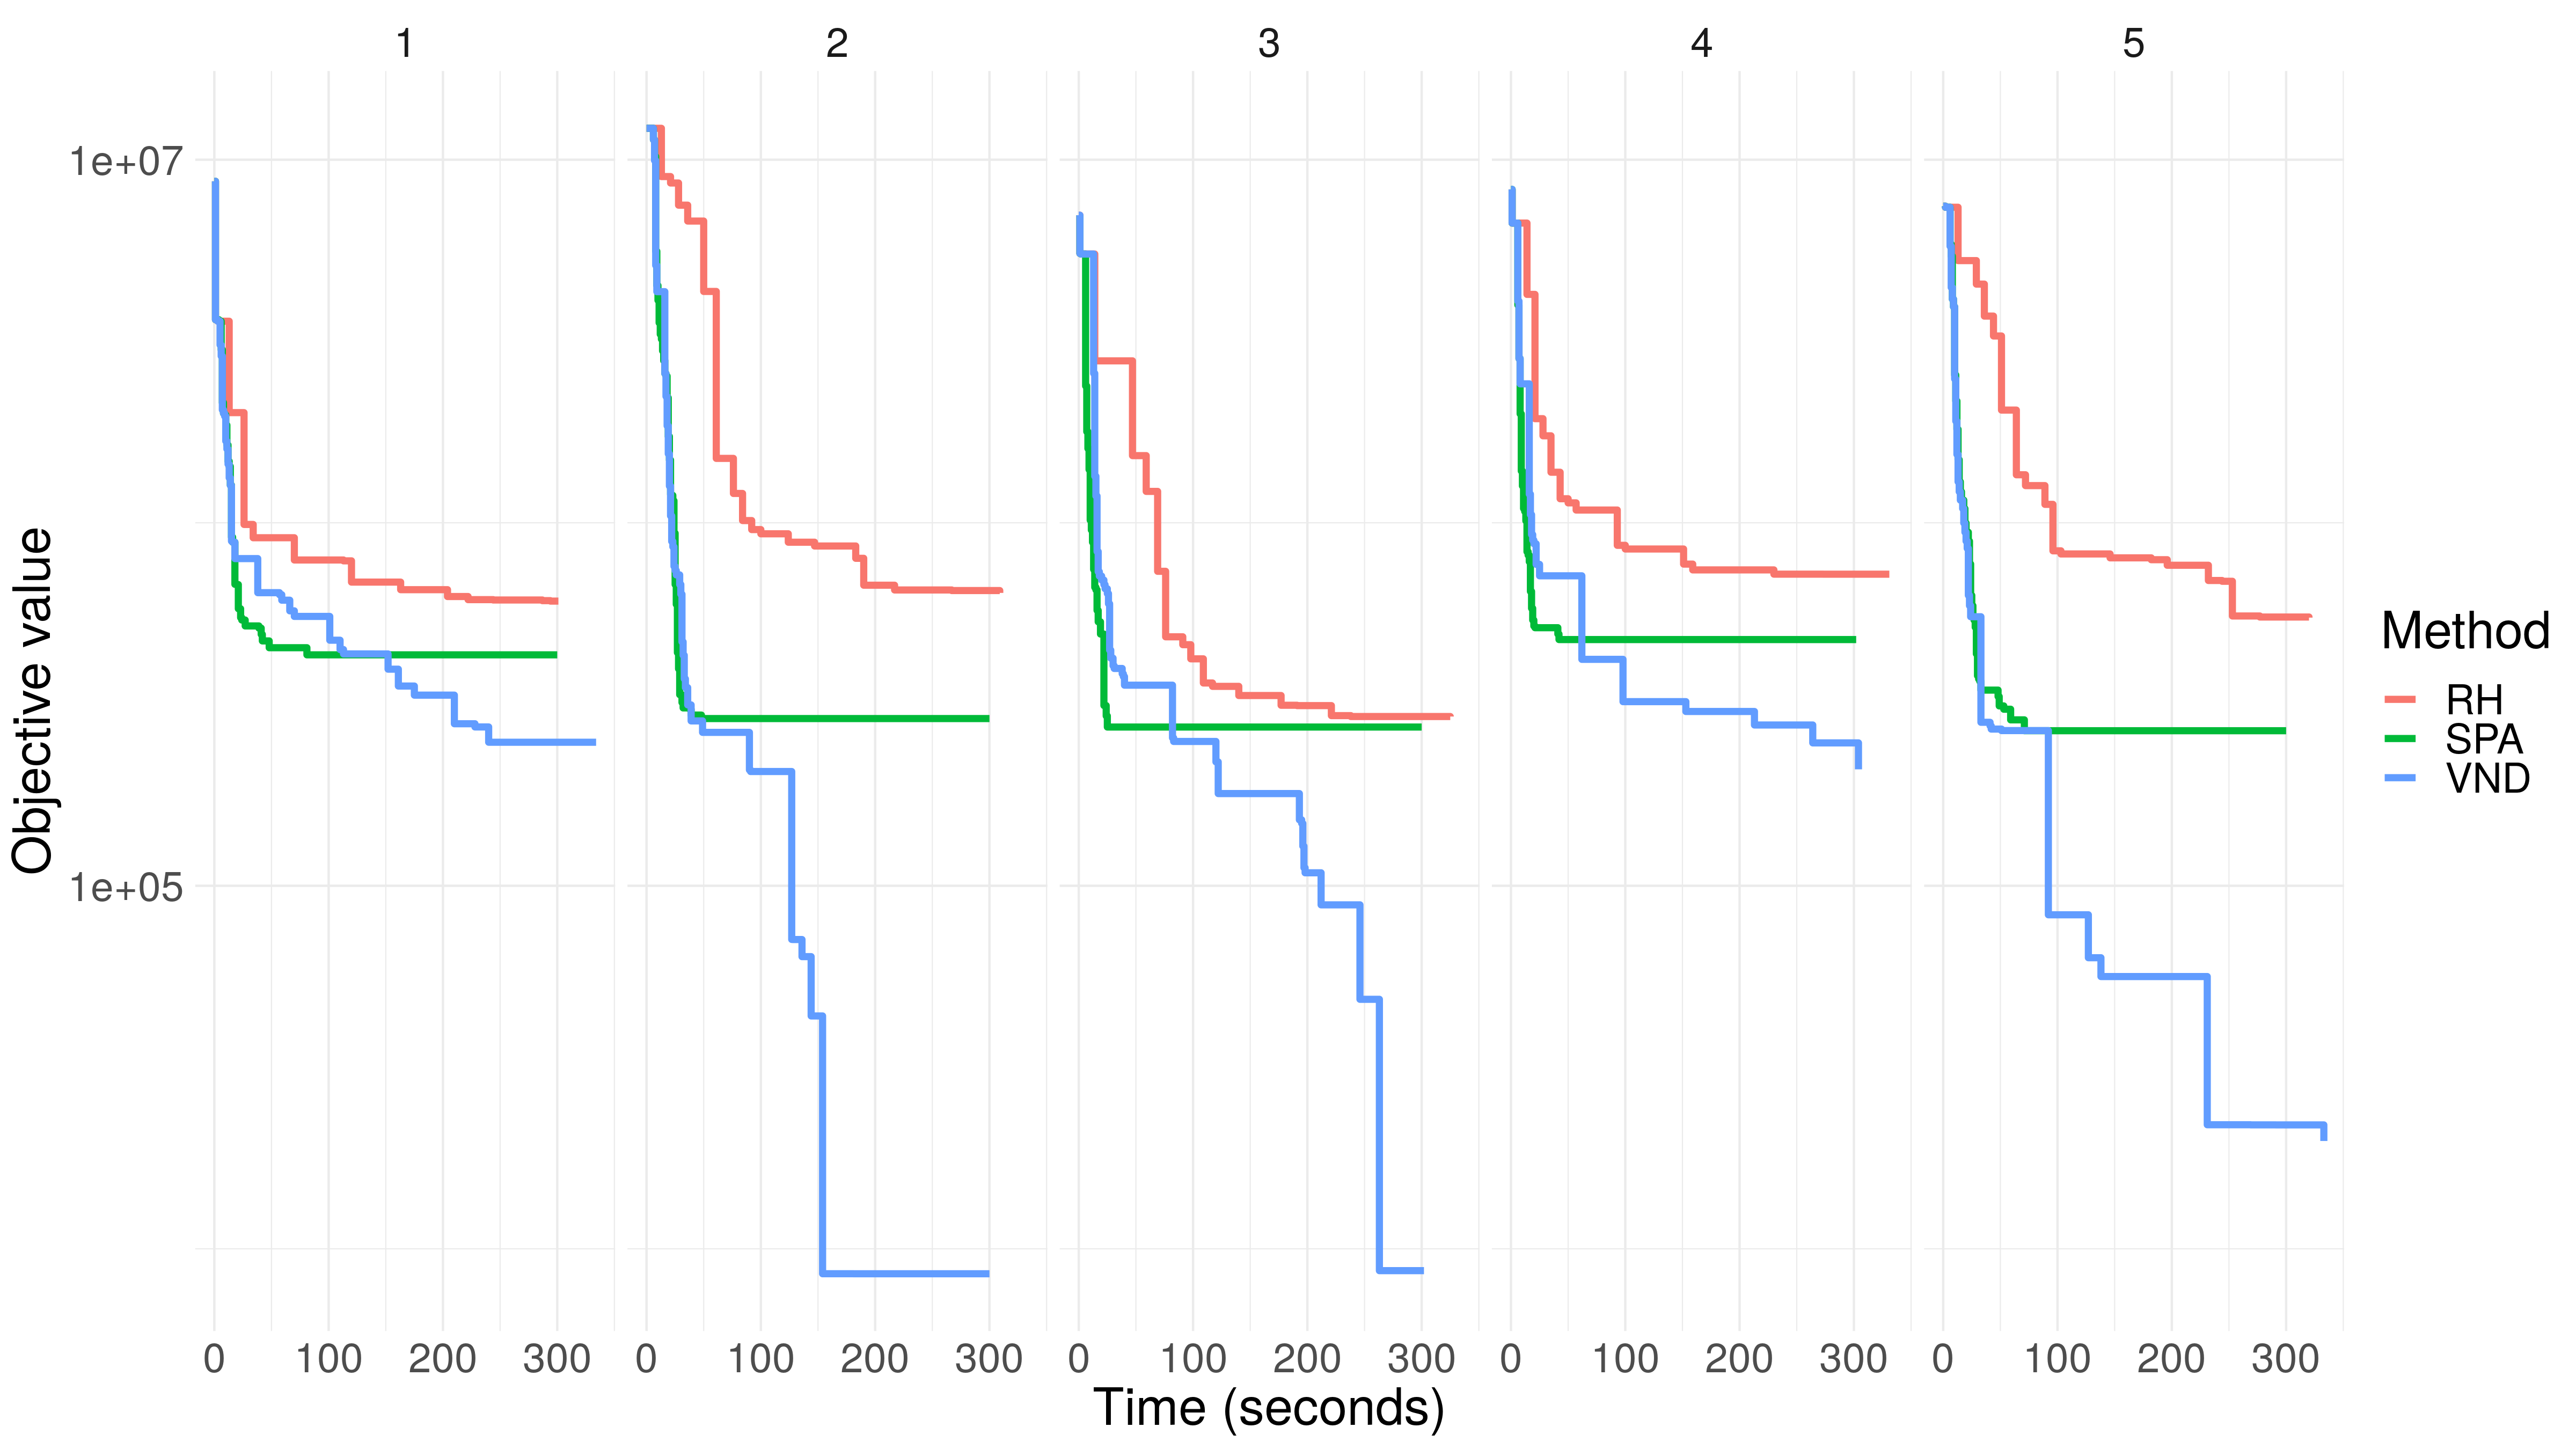
\includegraphics[width=\linewidth]{images/compare_neighbors.png}
\end{frame}

\begin{frame}
\frametitle{\textbf{Results: large instances}}
  % TODO: Time in units
  % TODO: size of police
  % TODO: rename instances
  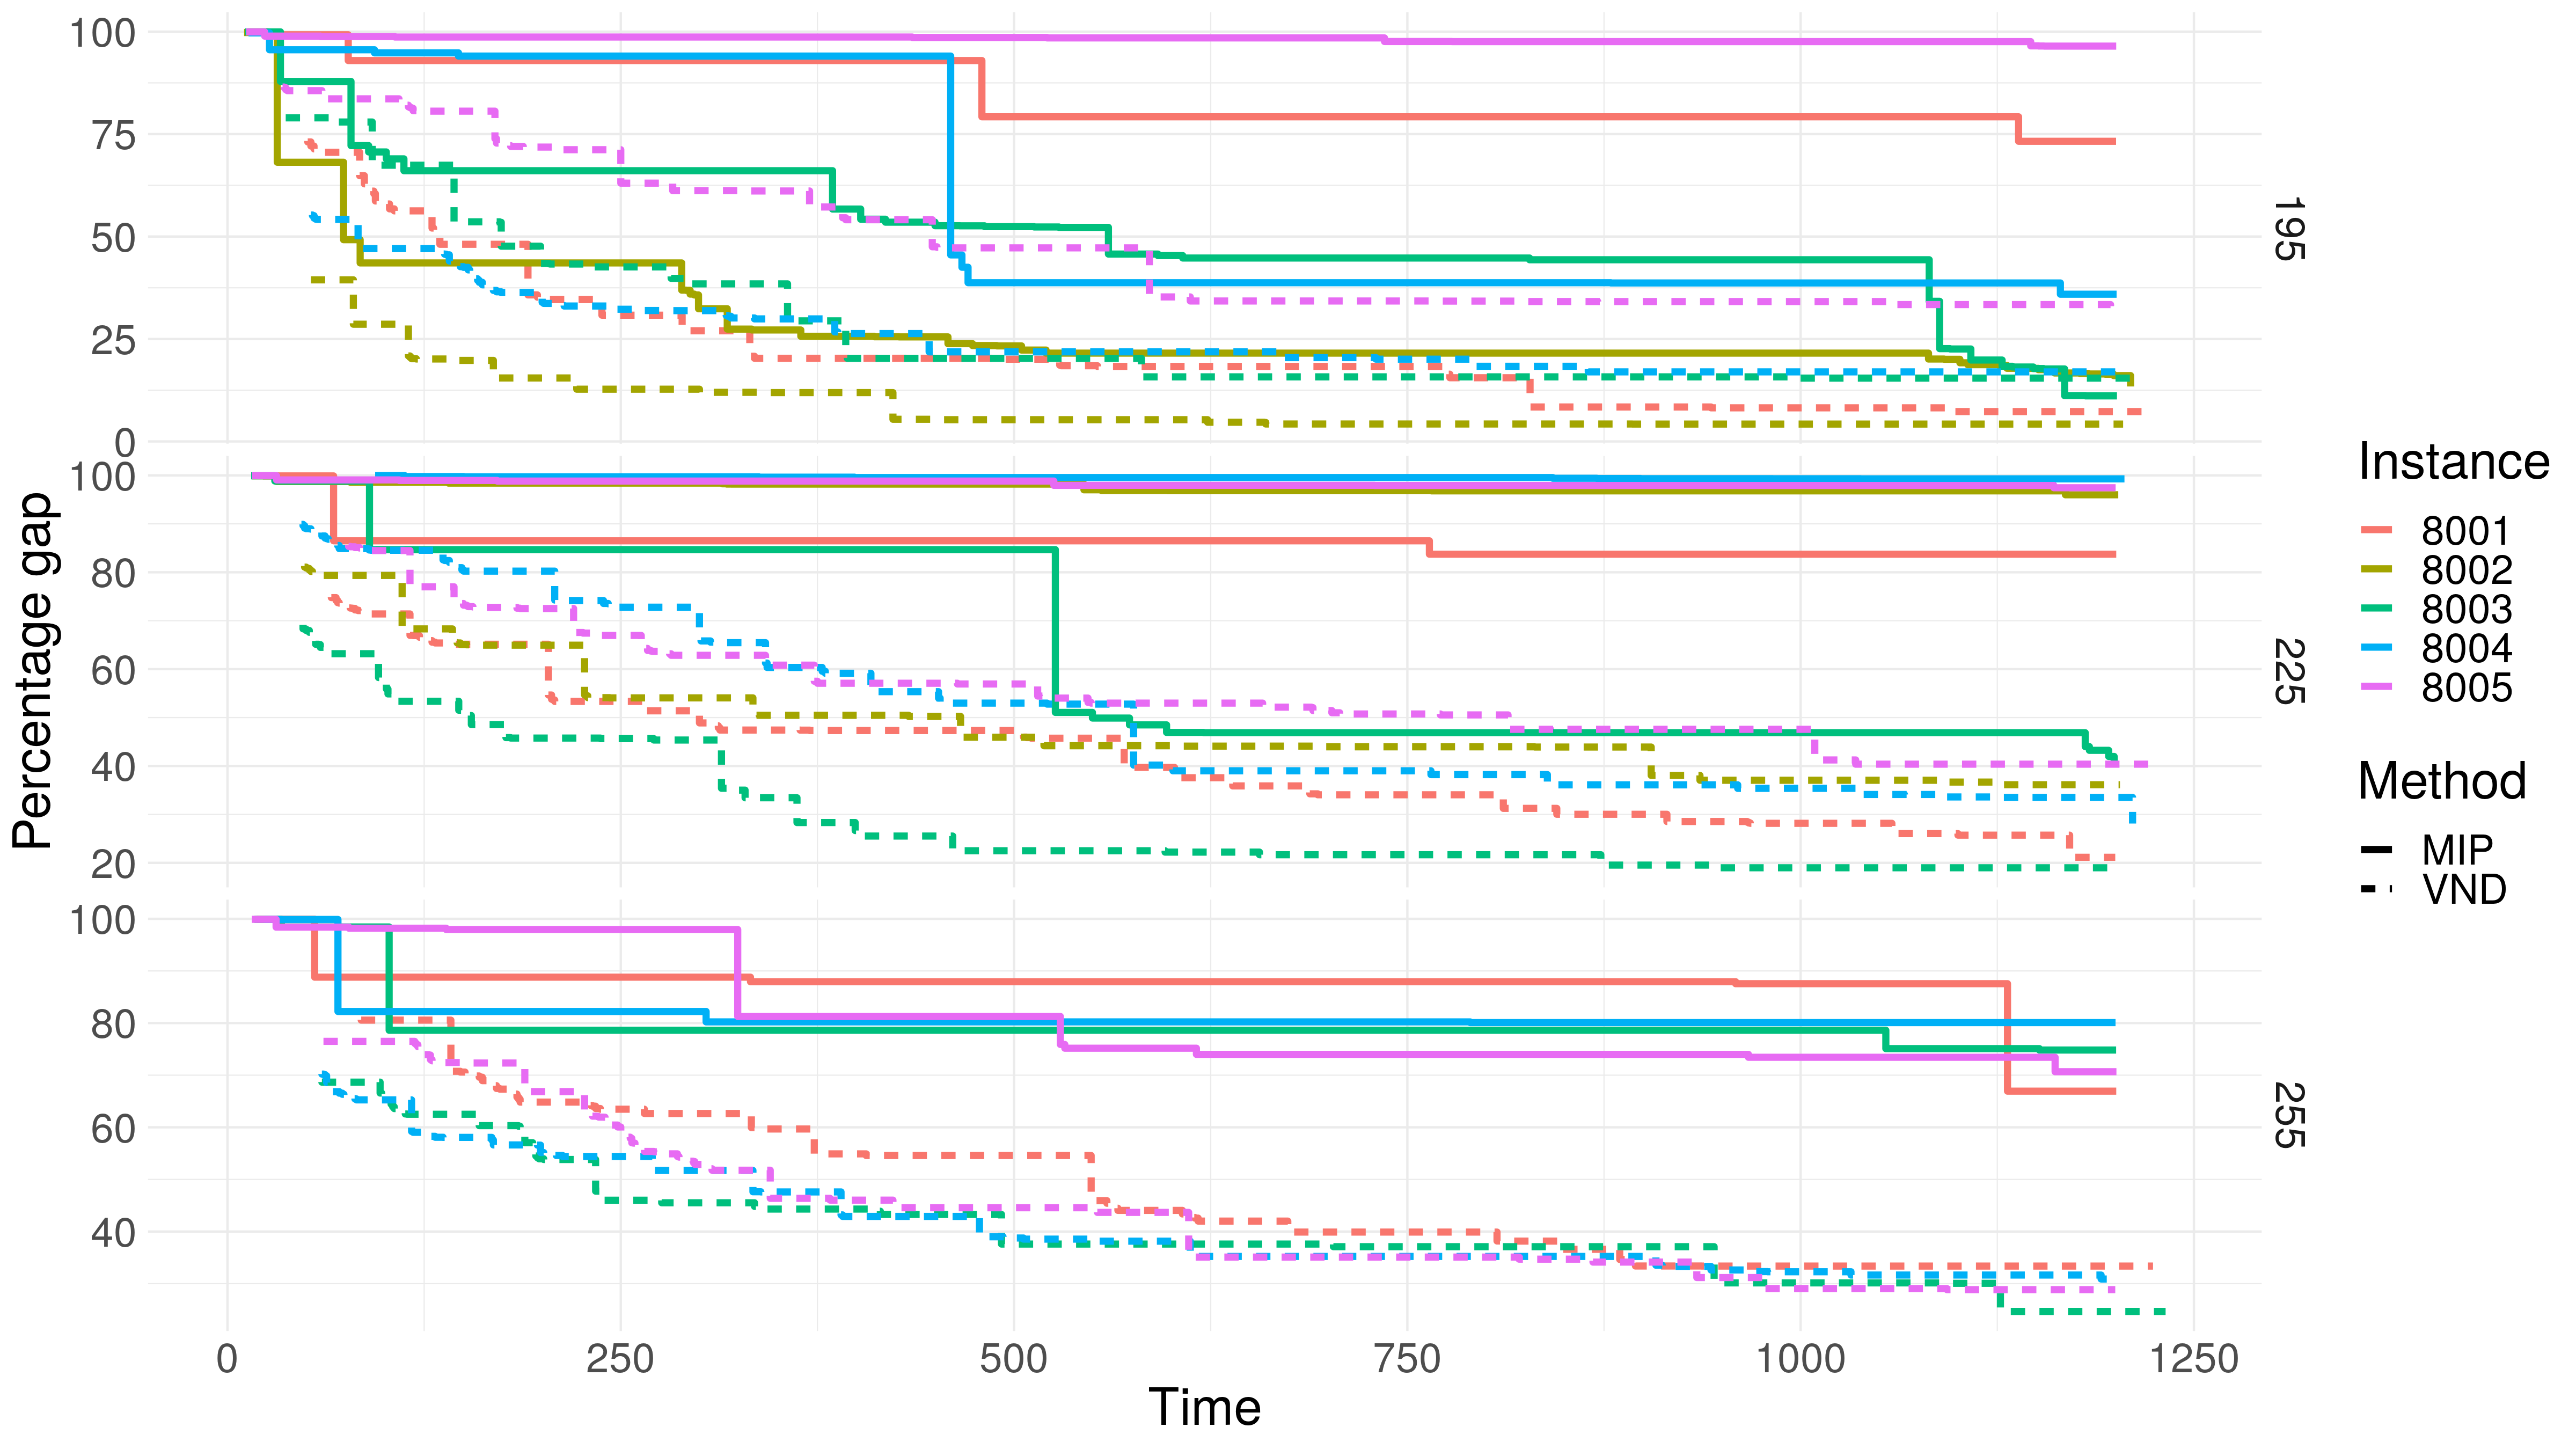
\includegraphics[width=\linewidth]{images/progress_gaps_very_large_255.png}  
\end{frame}

\begin{frame}
\frametitle{\textbf{Preliminary conclusions}}
  % TODO: check phrases
  % TODO: FMP and NRP: long?
  \pause
  \begin{block}{\textbf{Conclusions}}
    \begin{itemize}[<+->]
    \item \textbf{Graph representation} 
      built to efficiently explore the solution space of an aircraft.
    \item \textbf{Complementary neighborhoods} 
      are combined to efficiently explore the solution space.
    \end{itemize}
  \end{block}  
  \pause
  \begin{block}{\textbf{Perspectives}}
    \begin{itemize}[<+->]
      \item \textbf{Replace ad-hoc RH}
        e.g., by predicting / sampling promising patterns and running a set-covering model.
      \item \textbf{Apply graph in GRASP}
        by sampling paths in graph to quickly build solutions.
      \item \textbf{Generalize methodology}
        use it for the civil FMP problem or NRP.
    \end{itemize}
  \end{block}  
  
\end{frame}


  
\miniframesoff
  \begin{frame}[noframenumbering, plain]
    \frametitle{\textbf{Outline}}
    \setbeamercovered{transparent}
  \begin{enumerate}
    \transparent{0.3}
    \item \introtitle
    \item \firsttitle
    \item \secondtitle
    \item \thirdtitle
    \transparent{1}
    \item \textbf{\conclusiontitle}
  \end{enumerate}
  \end{frame}
\miniframeson

% \hypertarget{references}{%
% \section{References}\label{references}}

\end{document}
